%preamble - package inclusion and set up
\documentclass[12pt,twoside,a4paper,english]{report} %normalt 12pt!!!!
% Select encoding of your inputs
\usepackage[utf8]{inputenc}
% Make latex understand and use the typographic
% rules of the language used in the document.
%\usepackage[danish]{babel}
\usepackage[english]{babel}

% Use the vector font Latin Modern which is going
% to be the default font in latex in the future.
%\usepackage{lmodern}
\usepackage{mathptmx}

% Choose the font encoding
\usepackage[T1]{fontenc}

% Use color in tables
\usepackage[table]{xcolor}
\usepackage{pbox}
\usepackage{tabularx}
\usepackage{array}
\usepackage{multirow}

% Load a colour package
\usepackage{xcolor}
\definecolor{aaublue}{RGB}{33,26,82}  %<--define aaublue
\definecolor{white}{RGB}{255,255,255} %<--define white

% ref stuffz			original position
%\usepackage{cleveref}

% The standard graphics inclusion package
\usepackage{graphicx}

\makeatletter
  \g@addto@macro\@floatboxreset\centering %<--centering all figures
\makeatother

\usepackage{adjustbox}

% Set up how figure and table captions are displayed

\usepackage{float}
\restylefloat{figure}
\usepackage{caption}
\usepackage{subfigure}
\usepackage[subfigure]{tocloft}
\captionsetup
{
  %justification = centering,    %<--centering caption with multiple lines
  %justification = raggedright,  %<-- right alings caption with multiple lines
  justification = justified,  %<-- justify alings (make left and right side equal) caption with multiple lines
  font          = footnotesize, %<--set font size to footnotesize
  labelfont     = bf            %<--bold label (e.g., Figure 3.2) font
}
\captionsetup[subfigure]
{
  justification = centering, %<--centering subfigure caption text
  singlelinecheck=false,
  font = footnotesize        %<--font size for subfigures
} 

% Enable row combination in tables
\usepackage{multirow}

% Make space between table lines and text
\renewcommand{\arraystretch}{1.5}

% Enable commands like \st (strike out) and \hl (high light)
\usepackage{soul}

% Make the standard latex tables look so much better
\usepackage{array,booktabs}

% Enable the use of frames around, e.g., theorems
% The framed package is used in the example environment
\usepackage{framed}
\usepackage{colortbl}
\usepackage{longtable}
\usepackage{xcolor}
\usepackage{textcomp}

%-------MATHEMATICS---------------------------------
% Defines new environments such as equation,
% align and split 
\usepackage{amsmath}
\usepackage{relsize}
% Adds new math symbols
\usepackage{amssymb}
% Use theorems in your document
% The ntheorem package is also used for the example environment
% When using thmmarks, amsmath must be an option as well. Otherwise \eqref doesn't work anymore.
\usepackage[framed,amsmath,thmmarks]{ntheorem}
\usepackage{xifthen}%<--enables ifthenelse which is used in macros

\usepackage{siunitx} 
\sisetup{decimalsymbol=period}%<--\num{} will swich commas with periods
\sisetup{detect-weight}
%---------------------------------------------------

%-------PAGE LAYOUT---------------------------------
% Change margins, papersize, etc of the document
\usepackage[
  left=25mm,% left margin on an odd page %tidligere 25mm for baade right og left
  right=25mm,% right margin on an odd page
  top=35mm,
  ]{geometry}
  
% Modify how \chapter, \section, etc. look
% The titlesec package is very configureable
\usepackage{titlesec}
\makeatletter
\def\ttl@mkchap@i#1#2#3#4#5#6#7{%
    \ttl@assign\@tempskipa#3\relax\beforetitleunit
    \vspace{\@tempskipa}%<<<<<< REMOVE THE * AFTER \vspace
    \global\@afterindenttrue
    \ifcase#5 \global\@afterindentfalse\fi
    \ttl@assign\@tempskipb#4\relax\aftertitleunit
    \ttl@topmode{\@tempskipb}{%
        \ttl@select{#6}{#1}{#2}{#7}}%
    \ttl@finmarks  % Outside the box!
    \@ifundefined{ttlp@#6}{}{\ttlp@write{#6}}}
\makeatother

\titlespacing{\chapter}{0pt}{0pt}{10pt}
\titlespacing{\section}{0pt}{0pt}{-5pt}
\titlespacing{\subsection}{0pt}{8pt}{-5pt}
\titlespacing{\subsubsection}{0pt}{6pt}{-10pt}

\titleformat*{\section}{\normalfont\Large\bfseries\color{aaublue}}
\titleformat*{\subsection}{\normalfont\large\bfseries\color{aaublue}}
\titleformat*{\subsubsection}{\normalfont\normalsize\bfseries\color{aaublue}}

\usepackage{titlesec, blindtext, color}
%\color{gray75}{gray}{0.75}
\newcommand{\hsp}{\hspace{20pt}}
\titleformat{\chapter}[hang]{\Huge\bfseries}{\thechapter\hsp\textcolor{aaublue}{|}\hsp}{0pt}{\Huge\bfseries}

% Change the headers and footers
\usepackage{fancyhdr}
\setlength{\headheight}{15pt}
\pagestyle{fancy}
\fancyhf{} %delete everything
\renewcommand{\headrulewidth}{0pt} %remove the horizontal line in the header
\fancyhead[RO,LE]{\color{aaublue}\small\nouppercase\leftmark} %even page - chapter title
\fancyhead[LO]{}
\fancyhead[RE]{} 
\fancyhead[CE]{}
\fancyhead[CO]{}
\fancyfoot[RE,LO]{\thepage}
\fancyfoot[LE,RO]{} %page number on all pages
\fancyfoot[CE,CO]{}

% change first page of all chapters header and footer to fancy style
\makeatletter
\let\ps@plain\ps@fancy
\makeatother

% Do not stretch the content of a page. Instead,
% insert white space at the bottom of the page
\raggedbottom

% Enable arithmetics with length. Useful when typesetting the layout.
\usepackage{calc}
%---------------------------------------------------

\usepackage{appendix}

%-------BIBLIOGRAPHY--------------------------------
%setting references (using numbers) and supporting i.a. Chicargo-style:
\usepackage{etex}
\usepackage{etoolbox}
\usepackage{keyval}
\usepackage{ifthen}
\usepackage{url}
\usepackage{csquotes}
\usepackage[backend=bibtex, isbn=false, url=false, eprint=false, doi=false, style=numeric, sorting=none]{biblatex}
\addbibresource{setup/bibliography.bib}
%---------------------------------------------------

%-------MISC----------------------------------------
%%% Enables the use FiXme refferences. Syntax: \fxnote{...} %%%
\usepackage[footnote, draft, english, silent, nomargin]{fixme}		%!!!! DRAFT OR FINAL?!?!?!?!11!! change later!	
%With "final" instead of "draft" an error will ocure for every FiXme under compilation.

%%% allows use of lorem ipsum (generate i.e. pagagraph 1 to 5 with \lipsum[1-5]) %%%
\usepackage{lipsum}

%%% Enables figures with text wrapped tightly around it %%%
\usepackage{wrapfig}

%%% Section debth included in table of contents (1 = down to sections) %%%
\setcounter{tocdepth}{1}

%%% Section debth for numbers (1 = down to sections) %%%
\setcounter{secnumdepth}{2}

\usepackage{tocloft}
\setlength{\cftbeforetoctitleskip}{0 cm}
\renewcommand{\cftpartpresnum}{Del~}
\let\cftoldpartfont\cftpartfont
\renewcommand{\cftpartfont}{\cftoldpartfont\cftpartpresnum}
%---------------------------------------------------

%-------DANSK SPROG---------------------------------

%\addto\captionsdanish{%
%	\renewcommand{\figurename}{figur}%
%	\let\figureautorefname\figurename%
%	\renewcommand{\tablename}{tabel}%
%	\let\tableautorefname\tablename%
%%	\renewcommand{\equationname}{ligning}%
%%	\let\equationautorefname\equationname%
%	\renewcommand{\chaptername}{Kapitel}%
%	\let\chapterautorefname\chaptername%
%	\renewcommand{\partname}{Del}%
%	\let\partautorefname\partname%
%	\renewcommand{\sectionname}{afsnit}%
%	\let\sectionautorefname\sectionname%
%%	\renewcommand{\thesubsection}{underafsnit}%
%%	\let\subsectionautorefname\thesubsection%
%	\renewcommand{\pagename}{side}%
%	\let\pageautorefname\pagename%
%}

%-------HYPERLINKS----------------------------------
% Enable hyperlinks and insert info into the pdf
% file. Hypperref should be loaded as one of the 
% last packages
\usepackage{nameref}
\usepackage{hyperref}
\usepackage{bookmark}
\hypersetup{%
	%pdfpagelabels=true,%
	plainpages=false,%
	pdfauthor={Author(s)},%
	pdftitle={Title},%
	pdfsubject={Subject},%
	bookmarksnumbered=true,%
	colorlinks,%
	citecolor=aaublue,%
	filecolor=aaublue,%
	linkcolor=aaublue,% you should probably change this to black before printing
	urlcolor=aaublue,%
	pdfstartview=FitH%
}

% ref stuffz		new position
\usepackage{cleveref}

\crefname{appsec}{bilag}{bilag}
%---------------------------------------------------



% remove all indentations
\setlength\parindent{0pt}
\parskip 5mm
\usepackage{verbatim}

\definecolor{Gra}{RGB}{230,230,230}

%creates a nice-looking C#-text
\newcommand{\CC}{C\nolinebreak\hspace{-.05em}\raisebox{.3ex}{\scriptsize\text \#} }

%enables multi column lists
\usepackage{multicol}

%enables code-examples
\usepackage{listings}

\definecolor{coolblue}{RGB}{32,95,128}
\definecolor{mygreen}{rgb}{0,0.6,0}
\definecolor{mygray}{rgb}{0.5,0.5,0.5}
\definecolor{mymauve}{rgb}{0.58,0,0.82}
\usepackage{textcomp}
\definecolor{listinggray}{gray}{0.9}
\definecolor{lbcolor}{rgb}{0.9,0.9,0.9}

%for c code
\lstdefinestyle{cstyle}{
  backgroundcolor=\color{lbcolor},
	tabsize=4,
	rulecolor=,
	language=C,
  basicstyle=\scriptsize,
  upquote=true,
  aboveskip={1.5\baselineskip},
  columns=fixed,
  showstringspaces=false,
  extendedchars=true,
  breaklines=true,
  prebreak = \raisebox{0ex}[0ex][0ex]{\ensuremath{\hookleftarrow}},
  frame=single,
  showtabs=false,
  numbers=left,
  captionpos=b,
  numbersep=5pt,
  numberstyle=\tiny\color{mygray},
  showspaces=false,
  showstringspaces=false,
  identifierstyle=\ttfamily,
  keywordstyle=\color[rgb]{0,0,1},
  commentstyle=\color[rgb]{0.133,0.545,0.133},
  stringstyle=\color[rgb]{0.627,0.126,0.941},
}
%for python code
\lstdefinestyle{pythonstyle}{
    backgroundcolor=\color{lbcolor},
    tabsize=4,
    rulecolor=,
    language=python,
    basicstyle=\scriptsize,
    upquote=true,
    aboveskip={1.5\baselineskip},
    columns=fixed,
    showstringspaces=false,
    extendedchars=true,
    breaklines=true,
    prebreak = \raisebox{0ex}[0ex][0ex]{\ensuremath{\hookleftarrow}},
    frame=single,
    showtabs=false,
    numbers=left,
    captionpos=b,
    numbersep=5pt,
    numberstyle=\tiny\color{mygray},
    showspaces=false,
    showstringspaces=false,
    identifierstyle=\ttfamily,
    keywordstyle=\color[rgb]{0,0,1},
    commentstyle=\color[rgb]{0.133,0.545,0.133},
    stringstyle=\color[rgb]{0.627,0.126,0.941},
}
%for matlab code
\lstdefinestyle{matlabstyle}{
    backgroundcolor=\color{lbcolor},
    tabsize=4,
    rulecolor=,
    language=Matlab,
    basicstyle=\scriptsize,
    upquote=true,
    aboveskip={1.5\baselineskip},
    columns=fixed,
    showstringspaces=false,
    extendedchars=true,
    breaklines=true,
    prebreak = \raisebox{0ex}[0ex][0ex]{\ensuremath{\hookleftarrow}},
    frame=single,
    showtabs=false,
    numbers=left,
    captionpos=b,
    numbersep=5pt,
    numberstyle=\tiny\color{mygray},
    showspaces=false,
    showstringspaces=false,
    identifierstyle=\ttfamily,
    keywordstyle=\color[rgb]{0,0,1},
    commentstyle=\color[rgb]{0.133,0.545,0.133},
    stringstyle=\color[rgb]{0.627,0.126,0.941},   
}

%for java code
\lstdefinestyle{javastyle}{
	backgroundcolor=\color{lbcolor},
	tabsize=4,
	rulecolor=,
	language=Java,
	basicstyle=\scriptsize,
	upquote=true,
	aboveskip={1.5\baselineskip},
	columns=fixed,
	showstringspaces=false,
	extendedchars=true,
	breaklines=true,
	prebreak = \raisebox{0ex}[0ex][0ex]{\ensuremath{\hookleftarrow}},
	frame=single,
	showtabs=false,
	numbers=left,
	captionpos=b,
	numbersep=5pt,
	numberstyle=\tiny\color{mygray},
	showspaces=false,
	showstringspaces=false,
	identifierstyle=\ttfamily,
	keywordstyle=\color[rgb]{0,0,1},
	commentstyle=\color[rgb]{0.133,0.545,0.133},
	stringstyle=\color[rgb]{0.627,0.126,0.941},
}

%for inline c, syntax: \cline{ codeHere(); }
\lstdefinestyle{cinline}{
    style=cstyle,
    basicstyle=\small,
}
\newcommand\inlinec[1]{ \lstinline[style=cinline]{#1} }

%for inline python, syntax: \pythonline{ codeHere(); }
\lstdefinestyle{pythoninline}{
    style=pythonstyle,
    basicstyle=\small,
}
\newcommand\inlinepython[1]{ \lstinline[style=pythoninline]{#1} }

%for inline matlab, syntax: \matlabline{ codeHere(); }
\lstdefinestyle{matlabinline}{
    style=matlabstyle,
    basicstyle=\small,
}
\newcommand\inlinematlab[1]{ \lstinline[style=matlabinline]{#1} }

\usepackage{enumitem}
%\usepackage[citestyle=authoryear,natbib=true]{biblatex}

% Figures - TIKZ
\usepackage{tikz}
\usepackage[americanresistors,americaninductors,americancurrents, americanvoltages]{circuitikz}

% Wall of text logo
\newcommand{\walloftextalert}[0]{\includegraphics[width=\textwidth]{walloftext.png}}

\usepackage{pdfpages}
\usepackage{lastpage}
\usepackage{epstopdf}

\setlength{\headheight}{21pt}

\hfuzz=\maxdimen
\tolerance = 10000
\hbadness  = 10000

\usepackage{siunitx}
\graphicspath{{./figures/}}

%macros - please read this file
%Macro for 'where'-enviroment was improved by Andrea and Niels :-)

%-----------UNITS-------------------------------------------
\newcommand{\unit}[1]{&& \left[\si{#1}\right]}
%
%\newcommand{\unit}[1]{[\si{#1}]}            %<<| Use these if you want equations to be
%\newcommand{\eq}[2]{&&\si{#1} &= \si{#2}&&} %<<| centered.. .. will appear scrambled
%                                            %  | from one equation to the next though..
%                                            %  | and does not work with long equations.. :/
%
%-----------------------------------------------------------

%-----------WHERE ENVIRONMENT-------------------------------
\newenvironment{where}{\leavevmode{\parindent=1em\indent} Where:\\}{}
\newcommand{\va}[3]
{
  \begin{tabular}{p{20pt} p{40pt} p{290pt} l}
    & { $#1$ } & { #2 } & \ifthenelse{\isempty{ #3 }}  {}  {[{\si{#3}}]} \\
  \end{tabular}\\
}
%-----------------------------------------------------------

%-----------TikZ SETTINGS-----------------------------------
\tikzset{
  block/.style    = {draw, thick, rectangle,
                     minimum height = 2.1em,
                     minimum width = 1.7em},
  sum/.style      = {draw, circle, inner sep=3pt} %<--Adder
}
%-----------------------------------------------------------


%-----------Fanzy reference SETTINGS------------------------
%Figure references:
\newcommand{\figref}[1]{figure \ref{#1}}

%Figure references after full stop/period:
\newcommand{\Figref}[1]{Figure \ref{#1}}

%Table references:
\newcommand{\tabref}[1]{table \ref{#1}}

%Table references after full stop/period:
\newcommand{\Tabref}[1]{Table \ref{#1}}

%Section references:
\newcommand{\secref}[1]{section \ref{#1}} % on page \pageref{#1}}

%Section references:
\newcommand{\Secref}[1]{Section \ref{#1}} % on page \pageref{#1}}

%Subsection references:
\renewcommand{\subref}[1]{section \ref{#1}} % on page \pageref{#1}}

%Subsection references:
\renewcommand{\Subref}[1]{Section \ref{#1}} % on page \pageref{#1}}

%Appendix references:
\newcommand{\appref}[1]{appendix \ref{#1}} % on page \pageref{#1}}

%Appendix references:
\newcommand{\Appref}[1]{Appendix \ref{#1}} % on page \pageref{#1}}

%chapter references: 
\newcommand{\chapref}[1]{chapter \ref{#1}} % on page \pageref{#1}}

%chapter references: 
\newcommand{\Chapref}[1]{Chapter \ref{#1}} % on page \pageref{#1}}

%Units:
%\newcommand{\unit}[1]{&& \left[\si{#1}\right]}

%Text:
\newcommand{\tx}[1]{\text{#1}}

%Equation references:
%1 equation:
\renewcommand{\eqref}[1]{equation (\ref{#1})}

%-----------------------------------------------------------





\begin{document}       % TIP: If you are using TeXstudio you can open
%\tableofcontents      %      the file by Ctrl+LeftClick on setup/macros.tex
%\pagebreak             %      If the file doesn't exist, you will be asked
					   %      weather or not you want to create it.
%\begin{center}
%	\vspace{5cm}
%	\Huge{Worksheets}
%\end{center}
%\clearpage

%||||||||||||||||||||||||||||||||||||||||||||||||||||||||||||||||
%|||||||                 Example Inputs                  ||||||||
%||||||||||||||||||||||||||||||||||||||||||||||||||||||||||||||||
%|||||||                                                 ||||||||
%			 \input{chapters/aFigureSample.tex}			 %|||||||
%			 \input{chapters/bTableSample.tex} 		     %|||||||
%			 \input{chapters/cEquationSample.tex}		 %|||||||
%			 \input{chapters/dTikzSample.tex}            %|||||||
%			 \input{chapters/eCodeSample.tex}            %|||||||
%|||||||                                                 ||||||||
%||||||||||||||||||||||||||||||||||||||||||||||||||||||||||||||||
%||||||||||||||||||||||||||||||||||||||||||||||||||||||||||||||||


%%% Prereport %%%
		\setlength\cftaftertoctitleskip{2pt}
		\setlength\cftafterloftitleskip{6pt}
		\setlength\cftafterlottitleskip{6pt}
%\selectlanguage{danish}
%\title{Something about the coolest preprocessing methods and nice results for IDP study}

%%% Frontmatter Settings %%%
		\pagestyle{empty} %disable headers and footers
		\pagenumbering{roman} %use roman page numbering in the frontmatter I II...
	%	\fancyfoot[RE,LO]{18??} %page number on all pages
		\fancyfoot[LE,RO]{\thepage}
		\fancyhead[LE,LO,RE,RO]{}

%%% Introductory Formalities %%%
%\includepdf[pages={1}]{formalities/frontpage.tex}
			\clearpage
\thispagestyle{empty}

\begin{figure}[H]
	\raggedleft
	
\includegraphics[width=0.2\textwidth]{figures/aaulogo-en.png}
\end{figure} 

\vspace{5 cm}

\begin{center}
	\begin{Huge}
		\textbf{Does Task-related FMRI Preprocessing Need a FIX?}\\
		\vspace{5 mm}
		3. semester Masters, Biomedical Engineering \& Infomatics - Fall $2018$\\
		\vspace{3 mm}
	\end{Huge}
	{\Large Project group: $18$gr$9411$} \\
	\vspace{1cm}
	\large{Christian Korfitz Mortensen, Martin Alexander Garenfeld}
\end{center}
\vspace*{\fill}

\begin{center}
	\line(1,0){400}
\end{center}

%\newpage
%
%\large{\textbf{Project period:}\\
%P7, Autumn 2017\\
%01/08/2017 - 20/12/2017\\
%
%\textbf{Project group:}\\
%17gr7404\\} %\fxnote{Input group number}
%
%
%\begin{center}
%	\Large{\textbf{Collaborators:}\\
%		\vspace{1.5cm}
%	\rule{10cm}{1pt}\\
%	Irene Uriarte \\
%	
%	\rule{10cm}{1pt}\\
%	Martin Alexander Garenfeld \\
%	
%	\rule{10cm}{1pt}\\
%	Oliver Thomsen Damsgaard \\
%	
%	\rule{10cm}{1pt}\\
%	Simon Bruun \\}
%\end{center}
%
%
%
%\large{\textbf{Supervisors:}\\
%Strahinja Dosen \\
%Jakob Lund Dideriksen \\
%Lotte N.S. Andreasen Struijk} \\
%\\
\newpage
			% <--- the frontpage
			\pagestyle{fancy}
%{\small
\strut\vfill % push the content to the bottom of the page
\noindent Copyright \copyright{} Aalborg University 2015\par
\vspace{0.2cm}

\noindent This report is compiled in \LaTeX, originally developed by Leslie Lamport, based on Donald Knuth's \TeX. The main text is written in \emph{Latin Modern} pt 12, designed by Bogusław Jackowski and Janusz M. Nowacki. 
%The document is compiled via the website \url{www.overleaf.com}, an online collaborative based \LaTeX-editor with instant preview, which enables multiple persons to edit the document simultaneously.
Flowcharts and diagrams are made using Microsoft Visio. 
\clearpage
%			%\begin{document} 
\thispagestyle{empty}
\begin{titlepage}
\begin{nopagebreak}
{\samepage 

\begin{tabular}{r}
\parbox{\textwidth}{  \raisebox{-15mm}{
\includegraphics[height=3cm]{figures/aaulogo-en.png}}
\hfill \hspace{2cm} \parbox{8cm}{\begin{tabular}{l} %4.90
{\small \textbf{\textcolor{aaublue}{{7\textsuperscript{th} Semester, Masters Project}}}}\\
{\small \textbf{\textcolor{aaublue}{School of Medicine and Health}}}\\
%{\small \textbf{\textcolor{aaublue}{Communication Technologies}}}\\ 
{\small \textbf{\textcolor{aaublue}{Biomedical Engineering and Informatics}}}\\
{\small \textcolor{aaublue}{Fredrik Bajers Vej 7A}} \\
{\small \textcolor{aaublue}{9220 Aalborg}} \\
%{\small \textcolor{aaublue}{\emph{http://www.sict.aau.dk/electronics-and-it}}}
\end{tabular}}}
\end{tabular}

\begin{tabular}{cc}
\parbox{7cm}{

\textbf{The effect of limb position on myoelectric prosthetic control using linear regression}
\\
\textbf{Theme: Biomedical signals and information}

\small{
\\
}


\parbox{8cm}{


\textbf{Project period:}\\
P7, Autumn 2017\\
01/08/2017 - 20/12/2017\\
   
\textbf{Project group:}\\
17gr7404\\ %\fxnote{Input group number}
  
\textbf{Collaborators:}\\
\rule{5cm}{1pt}\\
Irene Uriarte \\
\rule{5cm}{1pt}\\
Martin Alexander Garenfeld \\
\rule{5cm}{1pt}\\
Oliver Thomsen Damsgaard \\
\rule{5cm}{1pt}\\
Simon Bruun \\

\textbf{Supervisors:}\\
Strahinja Dosen \\
Jakob Lund Dideriksen \\
Lotte N.S. Andreasen Struijk \\
}\\


\textbf{Pages:} 0\\
\textbf{Appendixes:} b \\
%\textbf{Ekstra:} For projektkode: Se forord\\ %eks. en CD eller USB
\textbf{Completed:} 19/12/2017\\

\vfill } &
\parbox{7cm}{
  \vspace{.15cm}
  \hfill
  \begin{tabular}{l}
  {\textbf{Abstract}}\bigskip \\
  \fbox{
    \parbox{6.5cm}{\bigskip
     {\vfill{\small \lipsum[15]
%write real thing
something
     \bigskip}}
     }}
   \end{tabular}}
\end{tabular}} %\vspace{1cm}


\centering
\textit{Publication of this report's contents, including source references, may only happen in agreement with the authors.}\\
%\textit{Offentliggørelse af rapportens indhold, med kildeangivelse, må kun ske efter aftale med forfatterne.}\\


\end{nopagebreak}
\end{titlepage}
%\end{document} 			 % <--- the titlesheet - contains the synopsis!!
%%% Preface %%%
			\cleardoublepage
			
%			\lipsum[15]
%write real thing
something			 % <--- this is the abstract!!
\clearpage
			\chapter*{Preface}

\lipsum[9]

\pagebreak				% <--- the preface
%
%\input{contents/bBackground/title.tex}
\clearpage
			\pdfbookmark[0]{Table of Contents}{label: tableOfCentents}
			\tableofcontents
			\cleardoublepage


%%% Mainmatter Settings %%%
\pagenumbering{arabic} %use arabic page numbering in the mainmatter
\fancyhf{}
\fancyfoot[C]{\thepage} %\text{ of} \pageref{LastPage}			% ADD LABLE{LASTPAGE} TO LAST PAGE !!
\fancyfoot[RE,LO]{18gr9411}																								   %
\fancyhead[RE,LO]{}																												%% } consider fancyfoots
\fancyhead[RE,LO]{\color{aaublue}\small\nouppercase\leftmark} %even page - chapter title %
\pagestyle{fancy}


%---------------------------INPUTS-------------------------------

%\input{contents/statusText.tex}
\part{Problem Analysis}
\chapter{Introduction} \label{chap:Introduction}
To experience and live with chronic pain can be immensely debilitating for any individual, and the consequences of experiencing chronic pain has been linked to numerous physical and mental conditions: restrictions in mobility and daily activities, dependency of therapeutic drugs, anxiety, depression and a reduction in quality of life \cite{Dahlhamer2018,NationalCenterforHealthStatisticsHealth2011}. \\ More than 100 million Americans are estimated to live with chronic pain, manifesting an extraordinary amount of human suffering along with additional large economic societal expenditures, as cost of medical care and loss of wages and productivity are escalating  \cite{InstituteofMedicine2011,Davis2017}. Compared to other major health conditions the number of patients suffering from chronic pain outnumber the total of patients suffering from heart disease and stroke, diabetes and cancer, and these conditions often include pain as a contributing component \cite{NationalCenterforHealthStatisticsHealth2011}. \\
“An unpleasant sensory and emotional experience associated with actual or potential tissue damage, or described in terms of such damage”, is how the International Association for the Study of Pain defines pain \cite{Merskey1994}. The phenomenon of pain is a very complex composition of both psychological factors, personality traits and states, and cognitive, emotional, motivational, contextual and cultural variables. Pain can furthermore be defined as either acute or chronic. Acute pain is a healthy response making up a self defense mechanism to warn and protect the human organism from any potential or further harm. \cite{Davis2017,Brook2011,Garland2013} Contrary to acute pain, chronic pain is not linked to organ damage of any kind, and does therefore not serve any useful purpose to the human organism \cite{Schmidt1986}. \\
It still remains incredibly challenging to assess and treat pain, as the mechanisms causing the experience of pain are not yet fully understood \cite{Nielsen2008,Coghill2011}. This includes all neurological steps in the processing of pain - from the peripheral detection of a stimulus to the spinal cord transmission and brain processing, including the further descending relay of the pain experience \cite{Feizerfan2015}. A step towards getting a higher understanding of chronic pain is to examine the mechanisms involved in acute pain. A justification for this reasoning is that chronic pain often is transitioned from repetitive acute nociceptive stimulations that lead to neuroplastic changes. \cite{Feizerfan2015, Mcgreevy2012}\\
Multiple studies \cite{Davis2017,Coghill2003,Kim2004,Emerson2014} have shown that the perception and sensitivity to acute pain are disposed to a great extent of subjective variability, suggesting that a pivotal key in understating the brain mechanism during noxious stimuli is found in the individual differences between subjects. Additionally, an individual's sensitivity can vary substantially from day to day, despite being exposed to the same stimuli. In some instances the psychophysical rating reported by the patient can rather be seen as a bias of the various scales used for reporting, than actually reflecting an unbiased measure of the experienced pain. It can furthermore be difficult for the physician to evaluate the patient's experienced pain from a third-person perspective. \cite{Coghill2003} \\
To examine if there is an actual difference between individuals in brain activation during the experience of pain and if this activation is correlated with the self-reported experience of pain could provide useful insight in the study of pain. 

\chapter{Problem Analysis} \label{chap:Problem_analysis}

In the problem analysis chapter a theoretical overview of essential topics encapsulating the study of pain will be presented. First, the mechanisms involved in the experience of pain will be described, and how the metabolic response of brain activation can be translated into images. Subsequently, differences in the experience of pain between individuals will be outlined, along with the possible difficulties in interpreting the corresponding images. Lastly, different methods to counter these difficulties will be presented, thereby laying the foundation for understanding the problems faced when studying the differences in the individual’s experience of pain. 
\section{Processing of Pain in the Nervous System}

%The International Association for the Study of Pain has presented the following definition of pain: \textit{“Pain is an unpleasant sensory and emotional experience associated with actual or potential tissue damage, or described in terms of such damage”}. \cite{1} 
Pain is a complex subjective phenomenon, where sensory and reactive components along with cognitive elements are activated to refrain an individual from further and future similar damage. \\
When the body is exposed to noxious stimuli, whether it originates from external or internal afflictions, information about the damaging stimuli is transmitted through neural pathways and through the peripheral nervous system to the autonomic and central nervous system. This process of transmission of a damaging event related to the brain is called nociception. It is mediated by certain receptors called nociceptors attached to myelinated A$\delta$ and unmyelinated C fibers that terminate at the dorsal horn of the spine. Perception of pain occurs when stimulation of nociceptors is high enough to activate A$\delta$ fibers, which results in an acute experience of prickling pain. When the stimulation increases, C fibers are activated, which results in a more intense pain experience that remains after the stimulus has ceased. These two phases of pain experience are associated with acute noxious stimulus, where the first phase is referred to as fast pain, and is of moderate intensity and appears immediately after the stimulus. The second phase, which is known as slow pain, is not as localizable, appears after a longer delay and is more painful. Activation of nociceptors can happen from sufficiently intense mechanical, chemical or thermal stimulation. Nociceptor activation is also modulated by inflammatory and bio-molecular influences. However, it is also possible for individuals to experience pain without a measurable noxious stimulus and for individuals to undergo a damaging trauma without suffering any pain sensation. \cite{Garland2013} \\ 
As stated in The International Association for the Study of Pain’s definition of pain, not only somatosensory components are involved in the experience of pain, but also cognitive and emotional elements. Psychological processes are major elements in the perception and expression of pain and involve the individual’s attention to the painful infliction, the cognitive appraisal of pain and emotional and behavioral reactions. These factors may have increasing or decreasing effects on the perception of pain. \\
As mentioned, the activation of nociceptors is transmitted along axons in peripheral nerves to the dorsal horn of the spine. From here the information is sent up the spinal cord via the spinothalamic tract to the thalamus. The thalamus functions as a major transmission location for sensory information to the cerebral cortex. The neural pathways terminate in subdivisions of the thalamic nuclei, from where the information is relayed to different cortical and subcortical divisions, including regions of the cerebral cortex, amygdala, hypothalamus, periaqueductal grey and basal ganglia. Worth remarking is that the insula and anterior cingulate cortex seem to almost always be activated when nociceptors are stimulated. \cite{Tracey2007} These structures are what process somatosensory input and is outputting neural activation that affects nociception and pain perception. \cite{Garland2013} This means that the brain does not only passively receive sensory input, but in addition actively regulates the sensory transmission by influencing the dorsal horn of the spine through a descending modulation. The brain structures involved in this regulation include the same as mentioned along with the rostral ventromedial medulla and dorsolateral pons/tegmentum. \cite{Tracey2007} Thus, when determining the intensity of pain perception during noxious stimulus of an individual these brain structures are of great importance to examine. 


\section{Metabolic Response to Brain Activation} \label{sec:pain}

To further understand the origin of brain activation during the experience of pain and how this activity is modulated by the brain, a measure of brain activation is therefore needed. To get a measure of brain activation, the underlaying physiologic response is of great importance to understand. \\
The activation of a brain region starts with a neurological input containing information about the noxious stimuli \cite{Tracey2007}. The increased neurological activity affects local metabolism as processing of the signal requires adenosine triphosphate (ATP) consumption during e.g. the reception and reconstruction of the action potential. Thus, ATP starts to be processed, leading to a decrease in oxygen concentration and increase in waste products. Thereby, the metabolic need for oxygen increases. Subsequently, these changes occurring in the local tissue of the corresponding brain region activate a vasodilation, increasing the blood flow to that region to reestablish the local homeostasis. During this regulation a not yet fully understood phenomenon occurs, where more oxygenated blood than needed, to compensate for the offset, is delivered, which floods the local region with oxygenated blood. This response to the increased neural activity is known as the hemodynamic response. Thus, the hemodynamic response becomes an indirect measure of neural activity. \cite{Glover2011,Poldrack2011}  %The overall increase in neural activity in that specific region following the need for metabolic regulation thereby permits the measure of the hemodynamic response, hence becoming an indirect measure of the neural activity.
An example illustrating the hemodynamic response can se seen in \figref{fig:back:HRF}.

\begin{figure}[H]                 
	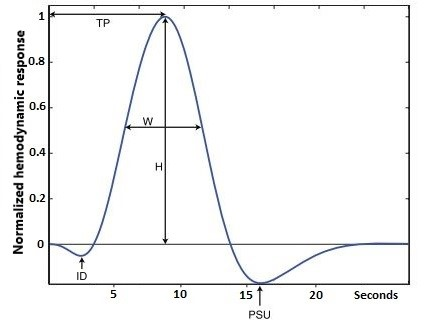
\includegraphics[width=.48\textwidth]{figures/aBackground/HRF}  
	\caption{A depiction of a single hemodynamic response curve. ID is the initial dip as less oxygen will be present as the metabolic demand increases, TP is time from stimulus until peak, W and H are the width and height of the response and PSU is a post stimulus undershoot. The illustration is modified from \cite{Poldrack2011}.}
	\label{fig:back:HRF} 
\end{figure}

\Figref{fig:back:HRF} is a representation of a perfect noiseless hemodynamic response curve to a brief stimuli. However, in reality the response is affected by physiological noise and is delayed in time compared to the stimulus onset. The peak height of the curve is commonly the most interesting feature of the response, as it portrays the amount of neural activity the best. The time to peak will often occur 4-6 seconds after stimulus onset. The duration of a response is approximately 20 seconds. There will furthermore be a noticeable initial dip of 1-2 seconds duration, when the initial oxygen reserves are used up and a 20 second poststimulus undershoot as homeostasis is reestablished. \cite{Poldrack2011}   

\section{Imaging of Brain Activation}

The metabolic changes associated with the hemodynamic response can be imaged through the use of fMRI \cite{Glover2011}. The following section will introduce the concept of fMRI and its use to study brain activation. Before reading this section, it is assumed that the reader is familiar with basic physics of nuclear magnetic resonance imaging and image reconstruction. If not, an overview can be found in the appendices \ref{sec:physics} and \ref{sec:IMrec}. \\
The fundamental factor that allows fMRI to image brain activity indirectly relies on the measure of the magnetic properties of blood. MRI is dependent on the magnetic susceptibility of the tissues. Local changes in susceptibility results in changes in the MR signal. \cite{Syed2015} Changes in susceptibility arise with the hemodynamic response as oxygenated hemoglobin $(HbO_2)$ is diamagnetic, and de-oxygenated hemoglobin $(Hb)$ is highly paramagnetic due to its four unpaired electrons, resulting in what is known as the Blood Level Oxygen Dependent (BOLD) contrast. Thus, as presented in the prior section, the increase in neural activity increases the blood flow to an extend greater than the metabolic utilization of oxygen, which results in a high $(HbO_2)$ to $(Hb)$ ratio. This makes up the difference in BOLD contrast. \cite{Glover2011,Poldrack2011,Khanna2015} \Figref{fig:back:bold} illustrates how the BOLD contrast is dependent on the amount of oxygenated hemoglobin. 

\begin{figure}[H]                 
	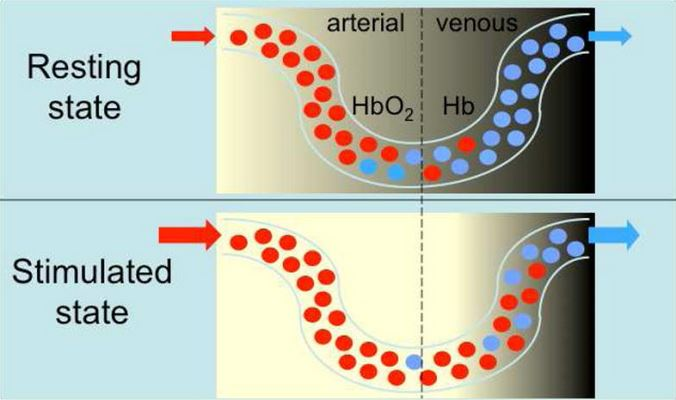
\includegraphics[width=.47\textwidth]{figures/aBackground/bold_response}  
	\caption{Illustration of the concentration difference in oxygenated $(HbO_2)$ and de-oxygenated hemoglobin $(Hb)$ during resting state and stimulated state. The diamagnetic properties of oxygenated blood changes the local magnetic substitutability facilitating a greater contrast change. Illustration taken from \cite{Glover2011}.}
	\label{fig:back:bold} 
\end{figure}

The changes in the BOLD contrast can be recorded by using a $T_{2}^*$ sequence, which is sensitive in detecting changes on the magnetic field, since the areas highly filled with oxygenated blood will result in a higher signal in the $T_{2}^*$-weighted sequence making these appear brighter in the reconstructed image. To capture the changes in blood flow over time the acquisitions have to be relatively fast. To achieve fast sequences, the result is a sacrifice of spatial resolution for temporal resolution, making it possible to acquire a whole brain volume in a couple of seconds. \cite{Khanna2015,Lee2002} \\ 
Other methods, as the arterial spin labeled (ASL) method exist for accentuating the functionality of the brain, but BOLD is favored, because it offers a high contrast to noise ratio. \cite{Lee2002} \\ As fMRI can be used as an indirect measure of the neurological response it can capture an individual’s brain activity associated to pain stimuli. Thus, fMRI can be used as a tool to facilitate the understanding of differences between individual’s pain perception.  
%As fMRI can capture the neurological response to pain through the hemodynamic response a measure to study the individual's response to pain is thereby derived. To know more of how the individual's perception of pain is measured in general and by fMRI, including the current difficulties, is of great significance.    

\section{Individual differences in pain perception and fMRI}
The study of individual differences is the investigation of an individual’s response to a similar intervention. This has been of great interest in medical fields as understanding individual pain experience would shape more precise treatments given the individual’s unique characteristics. However, understanding why individuals react differently across sensory modalities has for long been a perplexing problem. \\
In pain research, studies have shown a large variability in individual pain sensitivity as reported on a Visual Analogue Scale (VAS), when exposed to identical noxious stimuli \cite{Nielsen2008, Coghill2003}. This could indicate that individuals have different neurological responses to the same noxious stimuli, but on the other hand raise questions about the individual's integrity: is the subject over/underplaying the pain experience or engaging in drug seeking behavior? Thus, it has been of great interest to examine if the subjectively reported pain experience correlates with the actual neurological response in the individual. \cite{Coghill2011} Verifying a correlation between self-reports and brain activity during evoked pain stimulus would function as an important step in improving physician’s understanding of the mechanisms underlying individual differences in pain perception and the treatment of patients suffering from chronic pain. Brain imaging could in the future be an assistive tool to self-reports and behavioral evidence when assessing a patient’s claim regarding pain and physical condition. Such an addition would serve an especially valuable function when assessing patients unable to communicate verbally (e.g. young children or patients with dementia), patients with self-reports and behavioral evidence that are conflicting and for personalized pain management. In perspective, as brain imaging gets more accepted as an assistive tool in personalized pain management it will gain more interest in legal practices. Using it as proof or disproof on whether a patient is actually experiencing pain might affect financial outcome in insurance cases. However, due to ethical and jurisdictive circumstances it would be inappropriate to use it as an assistive tool in such cases until it has been sufficiently verified. \cite{Davis2017} \\
An indirect measure of functional brain response can be achieved through BOLD fMRI, and is often used to get a generic understanding of brain function in research. Averaging data across individuals is commonly applied to raise the signal-to-noise ratio. However, while providing a general knowledge on brain function, this practice excludes the possibility of observing brain function in the individual. The interest of examining individual differences in brain activity has been present for several years, but the technology has only been advanced enough during recent years for it to be carried out, due to higher magnetic field strength and faster acquisition time. This can be seen as more studies are using fMRI data acquired with 3.0 tesla scanners instead of 1.5 tesla scanners. \cite{Dubois2016} \\
%In 1999 and 2003 Coghill et al. \cite{Coghill1999, Coghill2003} published studies showing correlation between intensity of activation of specific brain regions associated with processing of noxious stimuli and subjects’ subjective pain sensitivity. Positron Emission Tomography (PET) scans and BOLD fMRI in a 1.5 tesla scanner was used respectively in the two studies for functional brain mapping. 
%However, as Dubois et al. \cite{Dubois2016} emphasize only during the recent years the MRI technology has been advanced enough to create images with sufficient SNR to use as means in studying individual differences. A review study by Wood et al. \cite{Wood2012} comparing 1.5 tesla and 3.0 tesla scanners, showed that using the BOLD fMRI technique can produce better susceptibility contrast sensitivity and due to the naturally higher SNR in 3.0 tesla scanners a 40 percentage increase in activation detection can be generated. \\
%In that relation, a validation of the 2003 study by Coghill et al. \cite{Coghill2003} with data from a 3.0 tesla scanner would be relevant, as a 1.5 tesla scanner was used for BOLD fMRI acquisition in \cite{Coghill2003}. Further reasoning for a validation study is that clinics tend to get higher tesla scanners installed, when desiring to get finer images in fMRI \cite{Wood2012}. Thus, the future of fMRI lies within the use of higher tesla scanners. In \cite{Coghill2003}, a total number of 17 subjects were included. To raise the reproducibility and verification in a validation study the number of participants included should be increased to examine if statistically significant result can be found in a higher sample size \cite{Dubois2016, Button2013}. \\
However, a downside of 3.0 tesla scanners compared to 1.5 tesla scanners is that various artifacts related to motion, respiration, bloodflow, pulsation of cerebrospinal fluid and air-tissue interfaces are more prominent \cite{Wood2012}. In that relation it would be beneficial to identify which concrete artifacts that are associated with BOLD fMRI along with which methods that exist to denoise the acquired images.   
%In that relation, examining different types of preprocessing methods to denoise the images would be of high interest. 

\section{Artifacts Associated with BOLD fMRI} \label{sec:noise}

When BOLD fMRI sequences are used to detect brain activity during in vivo experiments, not only task related activation will be present, as sources of noise  inevitably will impact the scan. \cite{Salimi-Khorshidi2014} The following section aims to identify the different artifacts associated with BOLD fMRI. \\
%Artifacts that usually influence the scan and thus the signal of interest are motion, respiration, blood flow/heart beat, pulsation of cerebrospinal fluid, air-tissue interfaces and scanner inhomogeneities.
As BOLD fMRI relies on very precise temporal and spatial placement, even millisecond or millimeter fluctuations caused by motion can have a large impact on the quality of the acquired signal. Motion does not only distort the brain in space but also disrupts the formation of the magnetic gradients that enables the BOLD signal to be detected correctly.Wholesale movement of the head, also called bulk motion, will cause the intensity of each voxel to change. As the maximum value of net magnetization in the direction of the magnetic field (M$_0$) is directly proportional to the number of spins in that voxel the BOLD signal will consequently be altered. In tissue interfaces such as white/grey matter boundaries, at the edge of the brain and around large vessels this is especially an issue. Furthermore, bulk motion will change the uniformity of the magnetic field as is has been tuned for a particular head position. This also directly affects M$_0$ and results in dropouts, reductions in signal intensity, in the BOLD signal and thus in the subsequent readout. Lastly, movement will change steady state magnetization, the relaxation back to equilibrium, by changing the time between excitations in the tissues that have moved from a slice to another. M$_0$ is affected until steady state has been reached again, and is referred to as the spin history effect. The spin history effect can cause the intensity of the BOLD signal to be detected as twice the level of the expected signal. \cite{Murphy2013} This will often result in an image where the intensities change in a striped pattern \cite{Poldrack2011}. \\
A typical protocol in pain research involves inducing noxious stimuli on the participant while recording the brain activity. These stimuli often causes the participant to move even more. During the movement some brain regions might also show activation associated with stimulus, while movement artifacts are present in the same time instance. Therefore it can be easy to mistake brain activation with stimulus correlated movement when analyzing the data, resulting in a weaker or even false statistical analysis. \cite{Poldrack2011} \\
Motion due to cardiac and respiratory cycles will cause the same artifacts as during bulk motion of the head. Additionally, cardiac pulsation and respiratory cycles will cause the brain stem to push the surrounding brain tissue. This will cause deformation and movement of cerebrospinal fluid that will form changes in M$_0$. Further artifacts can be found related to the frequency content of cardiac and respiratory cycles. The frequency of cardiac and respiratory cycles at rest are around 1 Hz and 0.3 Hz respectively. Relatively high-frequent compared to the BOLD signal of < 0.1 Hz. As the repetition time in a BOLD fMRI usually is 2-3 seconds, parts of the cardiac and respiratory cycles will be aliased into the BOLD signal’s frequency bandwidth. Thus, these artifacts can be mistaken for the BOLD signal when examining the frequency content. Another respiratory factor that affects the BOLD signal is the arterial level of CO$_2$. It works as a vasodilator and facilitates a global increase in the cerebral blood flow and thereby the BOLD signal. Thus, when a participant holds the breath hypercapnia arises and the BOLD signal increases, and during hyperventilation hypocapnia arises causing a decrease in the BOLD signal.  \cite{Murphy2013} This type of artifact might occur more when the participant is being subjected to noxious stimuli to attenuate the pain experienced. \cite{Poldrack2011}  \\
Furthermore, artifacts can form in areas where air and tissues meet, e.g. sinuses and the ear canals, and is caused by the main magnetic field inhomogeneities the air-tissue interface produce. It will be visualized as dropouts in the brain region adjacent to the air-tissue interface. \cite{Poldrack2011} \\
It can be summarized that many sources of noise can alter and disguise the signal of interest. Thus, being able to separate signal sources from noise is of great importance before analysing BOLD fMRI data, to avoid making any conclusions based on spurious data.




\section{State of the Art in MRI Preprocessing} \label{art}

In \secref{sec:noise} the various types of corrupting noise was presented. Continuous efforts have been made to avoid, remove and limit the influence of artifactual contributors before the quantitative fMRI analysis. Regular standard preprocessing methods of rigid-body motion correction, spatial smoothing and temporal filtering, have for long been a part of the preprocessing toolbox \cite{Poldrack2011,Salimi-Khorshidi2014}. But as studies grow more complex, seek greater SNR and introduce greater noise sources associated with the newer scanners, the need for more complex and fitting cleanup tools to add to the preprocessing toolbox is present. \cite{Wood2012,Liu2006} \\
In noise removal of fMRI datasets, there are mainly two widely used approaches: one data driven and one model based \cite{Salimi-Khorshidi2014,Iraji2016}.  In the latter, acquired data is compared to a predefined model, such as in the general linear model. These methods include additional physiological recordings, e.g. heart rate and breathing cycle, and use these regressors of non interest to regress/filter out their contribution to the recorded fMRI dataset. \cite{Salimi-Khorshidi2014,Iraji2016,Monti2011} Data driven models instead draw upon the data within the dataset utilizing methods of principal component analysis (PCA) and independent component analysis (ICA). Data driven methods are ideal when no good existing model fits the data as they can analyze the data in more flexible way. Hence, they are able to identify new and unexpected noise components, which then can be made to fit the model, thereby laying the foundation for a model based noise removal. \cite{Iraji2016} \\
One of the most often referred to articles making use of a model based method is the RETROspective Image CORrection (RETROICOR), introduced by Glover et al. \cite{Glover2000}. By measuring the phases of respiratory and cardiac cycles and comparing these to the fourier terms of the fMRI scan, they showed that it was possible to find these physiologic noise contributions which was synchronized with the scan. These could then be out-filtered showing considerably lowered peaks in the frequency spectrum at 0.8 Hz for cardiac influence and 0.15 Hz for respiratory influence. \cite{Glover2000} \\
A limitation of the model based RETROICOR was its dependency on physiologic data being acquired from external devices. A study by Behzadi et al. \cite{Behzadi2013} surpassed this restriction by utilizing a proposed data driven model of Component based noise Correction (CompCor). Instead of relying on data from external measurement of physiological noise, the CompCor method uses a PCA derived from noise regions of interest (ROI) to describe the physiological noise. Two methods of determining noise ROI’s were introduced: one using anatomical data to identify voxels where no neurological activity is presumed, such as in white matter and cerebrospinal fluid (CSF), the other defining noise ROI’s from voxels with high temporal standard deviation (tSTD) as these were found to correspond to ventricles, edge-regions, and vessels. The first five components from the PCA were hypothesized to describe the variance of the noise, and were used to fit a general linear model as nuance regressors and thereby remove the noise influence. Both CompCor methods produced a significant reduction in physiological noise fluctuations compared to the RETROICOR for BOLD fMRI. In addition, the second CompCor method was able to reduce subject motion artifacts. Though in cases of both severe motion artifacts and physiological fluctuations the PCA might only be able to describe one of the factors, limiting its use. \cite{Behzadi2013} \\
Model based noise cleanup methods like RETROICOR depend on external physiological measurements, and both the PCA based method CompCor and RETROICOR mainly focuses on physiological noise. This suggest that methods which can incorporate a higher level of motion correction along with correction for MRI scanner artifacts might be of greater use. \\
ICA is another data driven model, building on the blind source separation paradigm, for source analysis of fMRI datasets and was first introduced in 1998 by Mckeown et al. \cite{Mckeown1998}. Since then, multiple studies \cite{Calhoun2001a,Deslauriers2017,Parkes2018,Du2018,Tohka2008} have used and developed the use of ICA further. ICA has proven to be a powerful tool in separating the different sources which in summation comprise the complete fMRI scan. By maximizing spatial independence and non-gaussianity, the data can be decomposed into components each consisting of an activation map and its corresponding time course. \cite{Salimi-Khorshidi2014} This facilitated the prospect of by visually inspecting the components, a discrimination between artifactual activation and task-related could be made. Tools for easy employment of the ICA has been presented by groups like the Oxford University Centre for Functional MRI of the Brain (FMRIB), who presented a program called Multivariate Exploratory Linear Optimized Decomposition into Independent Components (MELODIC) for fast ICA implementation. \cite{FMRIB2016} The possibility of visually inspecting and labeling components as either artifactual or of interest, lead to discussions on standardization and comparability, as labeling of components could be subjected to operator biasing. Studies in the likes of \cite{Salimi-Khorshidi2014,Griffanti2017}, have proposed ways to recognize different artifactual components, but these can be hard to utilize since every component will be different from another. Subsequently, automatic labeling algorithms have been made to increase the sensibility, reliability and reproducibility of fMRI studies. These have been made by training classifiers in recognizing and separating artifactual components. \cite{Tohka2008} \\
In 2014 Salimi-Khorshidi et al. \cite{Salimi-Khorshidi2014} introduced the FMRIB's ICA-based X-noiseifier (FIX), for automatic denoising of resting state and task-related fMRI data. This methods employ the use an initial standard processing followed by a spatial-temporal fastICA, hand labeling of training set, feature extraction of 180 features and a heracial classifier for classification. \cite{Salimi-Khorshidi2014} \\
The use of pattern recognition is an interesting proposal as it makes way for a standardized approach, and reduces the labor intense work of labeling all components.   

%Despite the present implemented solutions for noise removal, none of the following have, to the authors current knowledge, been used and tested for noise removal in pain activation associated studies. Because the experience of pain result in activation of multiple centers of the brain, along with great risk of stimulus related movements, it would be of profound interest to compare some of the available solution in this field.  

\chapter{Study Objective}

In summary, it would be beneficial for the understanding of chronic pain to gain further knowledge on the brain mechanisms associated with acute pain. As different individuals report a wide variety in pain sensitivity when given identical pain stimuli, an examination on if the subjective reports correlate with intensity in brain activation in brain regions associated with pain would be of high interest. When using 3.0 tesla MRI scanners to indirectly measure brain activity through BOLD fMRI sequences, more of the activity will be captured compared to using 1.5 tesla scanners. The images will on the other hand be more prone to contain noise. For this reason proper preprocessing is needed to separate noise from signal of interest before analyzing the images. During the recent years more preprocessing methods have been developed in the field of fMRI as alternatives to the standard method. One of these is FIX, which with the use of MELODIC has shown great noise removal capabilities in resting state fMRI. A comparison of FIX and the standard method, presented in \secref{art}, on a large set of subjects that underwent a noxious stimuli task would be of great interest in the field of pain research, as this could provide insight on the advantages/disadvantages of this preprocessing method. This introduces the study objective:

\begin{center}

\textit{Evaluate the performance of using the standard preprocessing pipeline compared to incorporating FIX in the pipeline for noise removal in images acquired with a BOLD fMRI sequence in the context of individual cerebral activation as response to noxious stimuli.}

\end{center}

From the study objective the following primary and secondary study questions are sought answered: 

\begin{itemize}
	\item Primary: Does incorporating FIX in the fMRI preprocessing pipeline generate a higher signal-to-noise ratio?
	
	\item Secondary: Is the detection of individual differences improved when using FIX preprocessed data compared to standard preprocessed data?
	   
	 
\end{itemize}



\part{Problem Solution}
\chapter{Methods}

The methods section serves purpose of presenting the study design, how the test data was acquired and document the implementation of the three preprocessing methods used for noise removal. First, a flowchart introducing an overview of the general processing pipeline will be given, see \figref{fig:meth:overview}. Afterwards, the data acquisition protocol and the subjects demographics will be presented. Subsequently the implementation of the standard preprocessing methods will be introduced, followed by the FSL FIX method. Finally, the statistical framework used for testing the performance of each preprocessing method is presented. 

\begin{figure}[H]                 
	\includegraphics[width=.37\textwidth]{figures/bMethods/Flowchart_intro}  
	\caption{Flowchart presenting an overview of the processing pipeline throughout the methods chapter. Initially the data is acquired and the brain is segmented and extracted from both a structural and functional scan. Afterwards the extracted brains are registered to each other and to a standard. Then the brain from the functional scan is run through the pipeline of each of the two preprocessing methods, and subsequently the results of noise removal from each pipeline is compared.}
	\label{fig:meth:overview} 
\end{figure}
 
\section{Project Protocol} \label{proto}
The data used in this project originates from an ongoing Individual Differences Project (IDP) at the Department of Anesthesia at Cincinnati Children’s Hospital Medical Center. In this section, information on the project design will be outlined, i.e. which criteria that were set for in/exclusion, what the stimuli design was and how the data was acquired. The IDP study design involved subjecting each participant to noxious auditory, cold and heat stimuli. However, as only the noxious heat stimuli will be analyzed in this project, only the heat stimuli design will be described. 

139 healthy participants between the ages of 14 and 44 years were enrolled with no discrimination of ethnicity. In \tabref{tab:demo} an overview of essential population demographics is presented. 

\begin{table}[H]
	\caption{Overview of population demographics.}\label{tab:demo}
	\begin{tabular}{llll} \hline
		& \textbf{Age, mean(std)} & \multicolumn{2}{c}{\textbf{Gender n(\%)}} \\ \cline{3-4}
		&                & Female          & Male           \\ \hline
		\begin{tabular}[c]{@{}l@{}}\textbf{Total}\\ (n = 139)\end{tabular}   & \multicolumn{1}{c}{28.40(7.31)}    & 82(58.99)       & 57(41.01)      \\
		\begin{tabular}[c]{@{}l@{}}\textbf{Training}\\ (n = 34)\end{tabular} & \multicolumn{1}{c}{28.00(6.10)}    & 22(64.71)       & 12(35.29)      \\
		\begin{tabular}[c]{@{}l@{}}\textbf{Test}\\ (n = 105)\end{tabular}    & \multicolumn{1}{c}{28.53(7.68)}    & 60(57.14)       & 45(42.86)      \\ \hline
	\end{tabular}
\end{table}

As the study involved fMRI scans, participants that suffered from claustrophobia or had any electronic or metallic implants were not able to participate. Further exclusion criteria were pregnancy, skin conditions or past skin damage on or near the site of the heat stimuli delivery and intake of medications that might have altered pain sensitivity or brain activation. The participants were able to withdraw from the study at any given time. Additionally, the study investigators were able to withdraw participants if the they declined to comply with the experiment protocol, if a drug or pregnancy test showed positive, if there was an identification of severe brain, neurological or psychological abnormalities or if the investigator assessed that it would be in the participant's best interest. \\
Before enrollment in the study, the participants received a consent document (including the guardians/parents for participants under 18 years). First when full comprehension of the information was demonstrated the participant and guardians/parents would be allowed to sign the document.

\subsubsection{Data acquisition} \label{ac} 

Heat stimuli was delivered on the left calf with a Medoc Pathway ATS 16 x 16 mm temperature stimulator, while the participant was in a MRI scanner for the recording of brain activity using a $T_{2}^*$ image sequence. For visualization of brain structures and spatial normalization of functional data high resolution a T$_1$-weighted structural scan was first obtained. Both scan sequences were acquired with a Phillips Achieva 3.0 T x-series MRI scanner with 32 head coils. MRI acquisition sequence specific information for both the structural and functional scan can be found in \tabref{tab:mri}.   

\begin{table}[H]
	\caption{MRI specification for the $T_1$-weighted structural scan and the $T_{2}^*$-weighted BOLD scan. RL, AP  and FH denote right-to-left, anterior-to-posterior and foot-to-head, respectively.}\label{tab:mri}
\begin{tabular}{lll}
	\hline
	& \textbf{Structural (T1)}                                     & \textbf{BOLD ($\mathbf{T_{2}^*}$)}                                                \\ \hline
	\textbf{TR:}                     & 10 ms                                                                         & 2000 ms                                                                       \\
	\textbf{TE:}                     & 1.8 ms (delta 2 ms)                                                           & 35 ms                                                                         \\
	\textbf{Echo Sequence:}          & Spin Echo                                                                     & Gradient Echo                                                                 \\
	\textbf{Number of echoes:}       & 4                                                                             & 1                                                                             \\
	\textbf{Flip angle:}             & 8\degree                                                      & 90\degree                                                     \\
	\textbf{Slice orientation:}       & Sagittal                                                                      & Transverse                                                                    \\
	\multirow{-2.75}{*}{\textbf{Field of View:}}          & \begin{tabular}[c]{@{}l@{}}200 mm RL \\ 224 mm AP \\ 256 mm FH\end{tabular} & \begin{tabular}[c]{@{}l@{}}240 mm RL \\ 240 mm AP \\ 136 mm FH\end{tabular} \\
	\textbf{Slice Thickness:}        & 1 mm RL                                                                       & 4 mm FH                                                                       \\
	\textbf{Acquisition voxel size:} & 1 mm AP x 1 mm FH                                                             & 3 mm RL x 3 mm AP                                                             \\
	\textbf{Number of slices:}       & 200                                                                           & 34                                                                            \\
	\textbf{Acquisition Matrix:}     & 256 x 224                                                                     & 80 x 80                                                                       \\ \hline
\end{tabular}
\end{table}
 
Each participant went through three different block designs consisting of three different heat stimuli runs with seven noxious heat stimuli in each. A theoretical overview of stimuli designs and their effect on the hemodynamic response can be found in \secref{sec:Stim}. Each heat run had a unique sequence of 10 seconds of noxious stimuli temperatures of 47\degree C or 48\degree C interleaved with resting periods of skin temperature (35\degree C) stimuli. The sequence of each of the three heat runs can be seen in \figref{fig:meth:stimdesign}. 
Following each noxious stimulus the participant was instructed in rating the pain intensity using a trackball/response device and a computer projected VAS, after which the participant could rest until the subsequent stimulus was delivered. The time course of each heat run followed the same pattern starting with a 20 seconds initiating resting period followed by seven stimulus and rating/resting periods of 2 seconds increasing ramp stimulus, 10 seconds plateau stimulus, 3 seconds decreasing ramp stimulus and 37-38 seconds rating/resting. This meant that the interval of stimuli onset was approximately every 40 seconds resulting in a frequency of 0.025 Hz. Thereby the stimuli frequency was above the range of 0 to 0.015 Hz; a frequency range where scanner noise is present \cite{Poldrack2011}.

% As this low-frequency drift will always be present, it is very crucial to consider the interval of which tasks or stimuli are performed to avoid the output being present in the noise range of $0$ to $0.015$ Hz. Therefore stimuli or tasks should be performed within intervals of $70$ s or less. \cite{Poldrack2011} \\ 

\begin{figure}[H]                 
	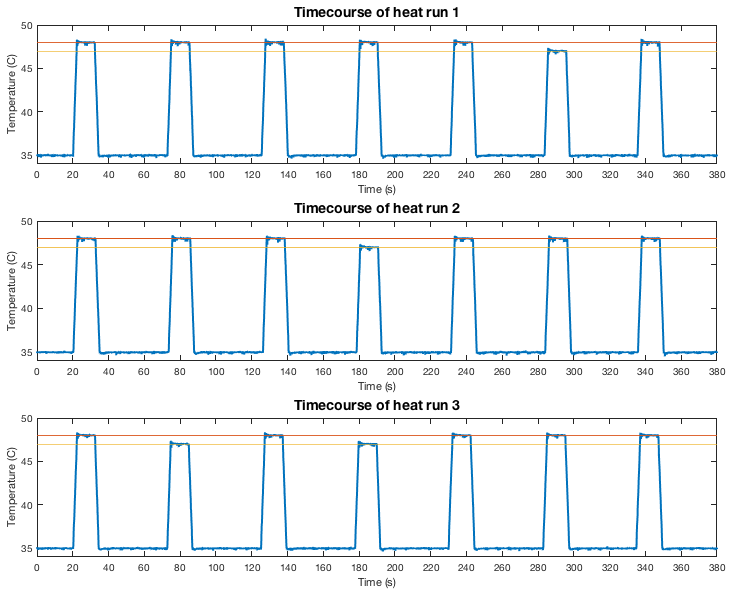
\includegraphics[width=.95\textwidth]{figures/bMethods/Stim_design} 
	 \caption{Illustrations of the time courses of heat stimuli for all three heat runs. The blue graphs depict the temperature of the heat stimuli and the yellow and red lines are used to distinguish between 47 and 48\degree C. In the first heat run the 47\degree C stimulus was delivered as the 6th stimulus, in the second as the 4th stimulus and in the third as the 2nd and 4th stimuli. The remaining stimuli were of 48\degree C.}
	\label{fig:meth:stimdesign} 
\end{figure}

To minimize bias all participants received identical stimuli in a single-blind fashion. Furthermore, the heat runs were induced in a pseudo-random order to confine the effects of habituation and expectation. Only the neurological response acquired during the 48\degree C stimuli was of interest in this project. 
 

\section{Brain Extraction and Registration} \label{BET}

In order to study activation in the brain, the brain has to be segmented and extracted from the surrounding tissue. To achieve an image only containing the brain, there was made use of the FSL Brain Extraction Tool (BET).  BET was used for extracting the brain in both the structural T$_1$-weighted image and in the functional T$_{2}^*$-weighted image sequence. As this is a standard applied method and is done before the implementation of preprocessing methods, it is seen non essential for the focus of this project. Hence, no further documentation of this step will be presented. For further documentation of BET specifications we refer to Smith et al. \cite{Smith2002}.    \\
The next step of preparing the functional images for analysis was to obtain the same coordinate system for these and the structural images. This step is called registration and is also known as spatial normalization. There are two levels of registration: intra-subject and inter-subject. Intra-subject is registering different scan sequences within the same subject and is done to spatially localize the activation. As the functional images contain very low resolution the localization of activation it can be hard to assess and therefore activation localization can more easily be studied by registering the functional image with a structural image. Inter-subject is to obtain the same brain localization in the coordinate system, called common space, for all participants. This is done to achieve population analysis, which facilitates result to be interpreted and reported objectively and consistently across studies. Inter-subject registration can be fulfilled by registering the brain for each participant to the often used Montreal Neurological Institute (MNI) template. \cite{Hajnal2001} \\
In this project a two step registration was implemented. First, a intra-subject registration was completed by registering the functional to the structural by utilizing the FSL FMRIB'S Linear Image Registration Tool (FLIRT), which uses affine linear transformation. \cite{Jenkinson2001} Secondly, a inter-subject registration was implemented, registering the structural for all participants to the MNI template. This was achieved by implementing both FLIRT and FMRIB'S Non-linear Image Regristration Tool (FNIRT), which uses non linear transformation. \cite{Andersson2007}   


\section{Dataset Structuring}

As presented earlier the total number of subjects included in this study was 139. Each subject underwent 3 heat runs where, for each, a functional scan was acquired, summited to a total of 417 scans. In \secref{art} it was introduced that the FIX preprocessing method utilizes a classification algorithm for separating noise sources from signal sources. The FIX software package comes with predefined training sets for training the classifier, but none of these have been made from fMRI scans consisting of signal related to the pain response from a noxious stimulus block design. Therefore, it was chosen to split the total dataset into a training dataset for training the classifier for this specific application and a test dataset for evaluating the performance of both preprocessing methods. \\
The training data set consisted of 34 subjects making a total of 102 scans\fxnote{ELABORATE ON THIS BEING SUFFICIENT, INSERT CITATION, \cite{Salimi-Khorshidi2014} suggest that a minimum of 10 subjects}. However, during the initial analyses two heat scans were found to have missing data resulting in the exclusion of these. This meant that the test dataset consisted of the remaining 105 subjects. In the test dataset 7 scans were found to have missing information or incomplete data, resulting in the exclusion of these. Therefore, the test dataset consisted of a total of 308 scans.  

 
\section{Standard Preprocessing}

Following the MRI data acquisition there are several steps, which need to be taken, before the multidimensional images are ready to undergo statistical analysis. These steps involves correction methods, which are often referred to as preprocessing. There are multiple steps in preprocessing fMR images depending on the apparent application and outcome intended. However, there is a standard set of methods that is usually used across all applications. \cite{Moayedi2018} The standard basic approach to preprocessing of task-related fMRI that defines a baseline for noise removal will in the following section be described. The steps that goes in to the standard preprocessing pipeline can vary depending on the defined study design. \fxnote{find citation}. In this project the standard preprocessing steps include: motion correction, slice timing correction, BET(Distortion correction??), spatial smoothing and temporal filtering. \Figref{fig:meth:std} provides a chronological overview over the implemented steps in the standard preprocessing pipeline.      

\begin{figure}[H]                 
	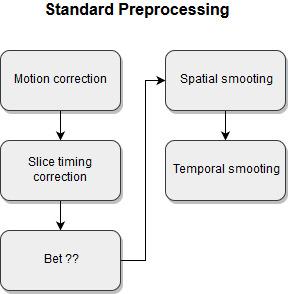
\includegraphics[width=.35\textwidth]{figures/bMethods/Standard_preprocessing} 
	\caption{Flowchart illustrating the steps in the standard preprocessing pipeline.}
	\label{fig:meth:std} 
\end{figure}

\subsection{Motion correction}

Correcting for motion artifacts when working with fMRI is nearly inevitable, since even the best subjects will not be able to hold still during acquisition. Even subtle movements as swallowing will be visible in the acquired image. \cite{Poldrack2011} To correct for these movement induced artifacts, a realignment of all volumes within a scan has been carried out using the FSL software program FMRIB's Motion Correction Linear Image Registration Tool (MCFLIRT). \cite{Jenkinson2002}
The tool was used to realign the series of images to a template image. The volume acquired halfway through the scan was used a reference image. This choice of template image is often justified by the middle volume being the closets to the average as well as the scanner at that time would have achieved maximum stability, as the magnetization would have reached steady state. \cite{Poldrack2011} A 6 degree of freedom transformation was used to realign the images, and can therefore only correct for bulk motion. \cite{Jenkinson2002}




\subsection{Slice timing correction}

When acquiring fMRI scans the slices in each volume are taken one by one. This can either be in an ascending, descending or interleaved order. Interleaved order is sequentially skipping every either odd or even slice and then afterwards acquiring the skipped slices. Ascending and descending is either from top to bottom or the opposite. Regardless of which order the slices were acquired, a misrepresentation of the hemodynamic response in each slice to the same hemodynamic response will be present due to the time difference in the slices. A representation of this effect can be seen in \figref{fig:meth:slice}. The difference in timing for each slice constitutes a problem when analyzing the data. The data is formed into statistical model, but since this model assumes that all slices are acquired at the same time point, the actual signal and the estimated in the statistical model creates a mismatch. \cite{Poldrack2011} \\

\begin{figure}[H] 
	{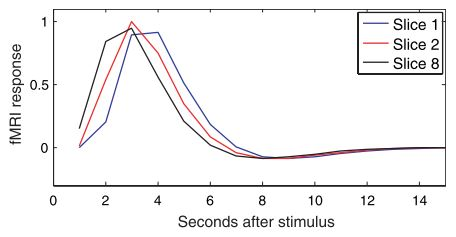
\includegraphics[width=.65\textwidth]{figures/aBackground/response}}  
	\caption{An illustration of the slice-wise acquisition effects the representation of the hemodynamic response. The response will seem to appear earlier in slice one compared to the others, as it is always the first acquired throughout the scan. \cite{Poldrack2011}}
	\label{fig:meth:slice}
\end{figure}

To account for the mismatch in the acquisition time of each slice, a correction has been implemented using FSL software \cite{FMRIB2018}. This is done by supplying the algorithm with acquisition order and the TR period. Hence, regular up and 2 second were inputed. The slice timing works by shifting the time series for the hemodynamic response curve for each slice in time to fit the middle of the TR period. This is achieved using Hanning windowed sinc interpolation. Choosing the middle slice as the reference, introduces the less interpolation, and is therefore seen as the most accurate method. \cite{Poldrack2011} Hence, the slice timing correction is carried out for each of the 193 volumes in a scan. 

%The standard algorithm for slice timing correction uses sinc interpolation between time points, which is accomplished by a Fourier transform of the signal at each voxel. The Fourier transform renders any signal as the sum of some collection of scaled and phase-shifted sine waves; once you have the signal in that form, you can simply shift all the sines on a given slice of the brain forward or backward by the appropriate amount to get the appropriate interpolation. There are a couple pitfalls to this technique, mainly around the beginning and end of your run, highlighted in Calhoun et. al below, but these have largely been accounted for in the currently available modules for slice timing correction in the major programs.
    

\subsection{Brain extraction}

This step is the brain extraction of the brain in the functional scan. The extraction of the functional brain is done in the same way as presented in \secref{BET}. 
\subsection{Spatial smoothing}

The next step in the standard preprocessing approach was to introduce spatial smoothing. Some of the image pixels will likely be contaminated with scattered noise presented higher pixel intensities. These can be removed by averaging the misrepresented pixel with its surrounding neighbors. Hence, this allows for the possibility of gaining a higher signal to noise ratio though with the consequence of a decrease in spatial resolution as the image gets blurred and smaller areas of activation gets smeared together. The operation can be justified by the closely neighboring voxel being correlated in effect to the hemodynamic response. Thereby some of the higher-frequency information removed by spatial smoothing. Furthermore spatial smoothing has the advantage that is reduces reduces the difference between subjects improving the between subject comparison. \cite{Poldrack2011} \\
The implementation of spatial smoothing on the data was done using the Smoothing over Univalue Segment Assimilating Nucleus (SUSAN) noise reduction filter in the FSL toolbox. The 3 dimensional spatial smoothing was carried out on each volume of the FMRI data set separately. Thereby reducing noise without reducing valid activation, which should be achieved using a mask size of 5 mm full width half maximum (FWHM), thus resulting in a trade off of smoothing bigger and smaller areas of activation. An advantage of the SUSAN algorithm is its ability to distinguish between tissue types as e.g. grey matter and white matter and thereby only including intensity value from neighboring voxels which consist of the same tissue type as the voxel being smoothened. Thereby all structures in the image should be preserved. \cite{Smith1997}  


\subsection{Temporal smoothing}

A characteristic noise which represents itself during fMRI data is the presence of a low-frequency drift. The drift is characterized as a slow increasing trend in the BOLD magnitude, when assessing the signal in the time domain. Doing a Fourier Transform, to analyze the signal in the power spectrum, would reveal low frequency contributers influencing the signal. As mentioned in \secref{ac}, the frequency of noise was 0 Hz to 0.015 Hz and the frequency band of activation is 0.01 Hz to 0.02 Hz. To dampen some of the low-frequency artifactual content a high pass filter with a cutoff frequency of 100 seconds (0.01 Hz) was implemented. \cite{FMRIB2018}. \\


 
 % The reason for this type of noise contamination has been heavily investigated, and conclusions state that the noise originates from MRI scanner instability. As this low-frequency drift will always be present, it is very crucial to consider the interval of which tasks or stimuli are performed to avoid the output being present in the noise range of $0$ to $0.015$ Hz. Therefore stimuli or tasks should be performed within intervals of $70$ s or less. \cite{Poldrack2011} \\ 
 
 
 
 


\section{FSL FIX}

The following section will describe the implementation of FIX, which introduces a faster and more standardized approach to ICA-based noise cleanup \cite{Salimi-Khorshidi2014}. The FIX method is a more extensive approach, which adds another layer of preprocessing to the standard preprocessing. This meant that before initiating FIX the data needed to undergo the exact same steps as in the standard preprocessing presented in \secref{sec:std}. Following the standard preprocessing, the functional scan underwent an ICA to split the sources in the acquired signal, which ideally would separate signal of interest from noise. Afterwards an analysis of optimal number components in which the data should be split was performed. The FIX tool uses a classifier to separate noise components from signal components. The classifier needed to be trained before it applied on a new data set. In \figref{fig:meth:fix} a flowchart showing the steps for both the training data set and the test data set in the FIX pipeline is illustrated. 


\begin{figure}[H]                 
	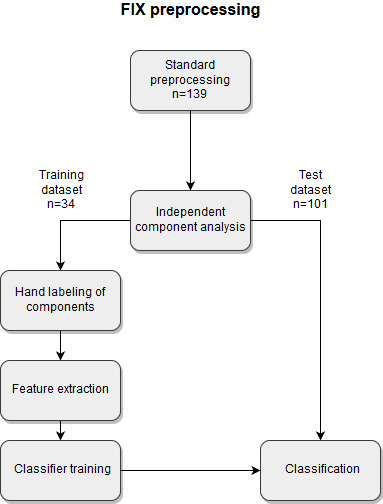
\includegraphics[width=.6\textwidth]{figures/bMethods/FIX_flow} 
	\caption{Flowchart illustrating the two datasets and the corresponding steps that was applied to each dataset in the FIX pipeline. Initially, MELODIC was used to estimate independent components. These components were subsequently hand labeled, and used to train the classifier along with 186 features extracted from each component. The trained classifier could then be used to identify the the source of each component from a test data set.}
	\label{fig:meth:fix} 
\end{figure}

%
%
%\subsection{Calculation of Independent Components}
%
% For a single session ICA the MELODIC FSL program utilizes the FastICA algorithm to obtain independent components. This section seeks to lay out how the FastICA algorithm works and which mathematical techniques that are exploited. \\
% As stated in \secref{sec:ICA}, from the central limit theorem we get that observed mixed signals tend to have a more Gaussian distribution than the individual source signals, since the observed signal is a summation of the source signals. As a result of this, an approach is to find a linear transformation that leaves the source signals as non-Gaussian as possible. This principle is what the FastICA algorithm is build up around. \\
% Firstly the vector \textbf{b} is introduced, which is a row vector in the mixing matrix \textbf{A}, and is used in a linear combination:
% 
% \begin{equation}
% y = \mathbf{b^T}\mathbf{x}
% \end{equation}
% 
% By substituting $\mathbf{x} = \mathbf{A}\mathbf{s}$ in the previous equation:
% 
% \begin{equation}
% y = \mathbf{b^T}\mathbf{A}\mathbf{s} = \mathbf{q^T}\mathbf{s}
% \end{equation}
% 
% Where $\mathbf{q^T} = \mathbf{b^T}\mathbf{A}$. From this it can be deduced that \textit{y} is an IC, when only one of the entries of \textbf{q} is non-zero and the rest is zero. This means that there is no addition of any random processes and the component will be as non-Gaussian as possible. An IC can then be obtained by calculating a value of \textbf{b} that maximizes the non-Gaussianity of the distribution of $\mathbf{b^T}\mathbf{x}$ as $\mathbf{b^T}\mathbf{x} = \mathbf{q^T}\mathbf{s}$. This gives an optimization problem with convergence at local maxima. As there exist a local maximum of the non-Gaussianity for both \textit{s} and ${s_i}$, the optimization landscape in a n-dimensional signal gives a total of \textit{2n} local maxima.
% To be able to optimize according to non-Gaussianity, a quantitative measure of such is needed. This can be provided by the fourth order cumulant, kurtosis, which is zero when \textit{y} is Gaussian distributed and non-zero when \textit{y} is non-Gaussian distributed (negative when sub-Gaussian and positive when super-Gaussian). Given this property and the central limit theorem, the linear combination $\mathbf{b^T}\mathbf{x}$ that yields an IC can be found at the local maxima of the absolute value of the kurtosis of \textit{y}. The kurtosis of \textit{y} is given by:
% 		
%\begin{equation}
%kurt(y) = E{y^4} - 3E{y^2}^2
%\end{equation}
% 		
%As the whitening of the data results in unit-variance, \textit{kurt(y)} can be modified to:
%		
%\begin{equation}
%kurt(y) = E{y^4} - 3
%\end{equation}
% 		
%To simplify the theoretical analysis furthermore the linear properties of kurtosis for sums of variables can be utilized. For two random variables, \textit{$x_1$} and \textit{$x_2$}, it holds that:
%
%\begin{equation}
%\begin{split}
%kurt(x_1 + x_2) &= kurt(x_1) + kurt(x_2) \\
%kurt(\alpha x_1) &= \alpha^4 kurt(x_1)
%\end{split}
%\end{equation} 			
%For the multiplicative scalar textit{$\alpha$} the kurtosis is non-linear, and the optimization problem can thus be written as:
% 			
%\begin{equation}
%kurt(y) = \sum_{i} q_{i}^{4}kurt(s_i)
%\end{equation}
% 			
%Due to the whitening of the data, where \textit{y} has unit-variance, a constraint is put on the vector \textbf{q}. Since $E{y^2} = \sum_{i}^{n} q_{i}^{4}$ the vector \textbf{q} is constrained to the unit-sphere. For the whitened data \textbf{z} a linear combination $\mathbf{w^T}\mathbf{z}$ that maximizes non-Gaussianity is sought for. From the fact that $\mathbf{q} = \mathbf{V}\mathbf{A})^{T}\mathbf{w}$, the following is given:
% 			
%\begin{equation}
%\parallel \mathbf{q} \parallel^{2}= (\mathbf{w}^{T}\mathbf{V}\mathbf{A})(\mathbf{A}^{T}\mathbf{V}^{T}\mathbf{w}) = \parallel \mathbf{w} \parallel^{2}
%\end{equation}
% 			
%This expresses that constraining the vector \textbf{q} to lie on the unit sphere equally constraints \textbf{w} to the unit sphere. The objective is now to find a value of \textbf{w} that maximizes the absolute value of the kurtosis of $\mathbf{w^T}\mathbf{z}$. Whitening further allows the linear combination $\mathbf{w^T}\mathbf{z}$ to be understood as projections on the line in a 1-D subspace spanned by \textbf{w}. What is sought for is the direction of \textbf{w} where the absolute value is maximized, which then makes out an IC. \\
%To solve this optimization problem a commonly used technique is the gradient algorithm to reach convergence at local maxima, thus calculating the direction where the absolute value of the kurtosis of $\mathbf{w^T}\mathbf{z}$ is growing most strongly. The can be computed as the following:
% 			
%\begin{equation}
%\frac{\delta|kurt(\mathbf{w^T}\mathbf{x})|}{\mathbf\delta\varTheta{w}} = 4 ~ sign ~ (kurt(\mathbf{w^T}\mathbf{z})[E{\mathbf{z}(\mathbf{w^T}\mathbf{z})^{3}} - 3\mathbf{w}\parallel\mathbf{z}\parallel ^{2}]
%\end{equation}
% 				
%However, there is in practice disadvantages associated with using the gradient algorithm, e.g. slow convergence rate and is dependent on a proper choice of learning rate. The fixed point algorithms is suggested as a faster algorithm alternative. At the stable point of the gradient algorithm, the gradient is pointing the direction of \textbf{w}. It is only in this case that \textbf{w} will not change direction when adding the gradient. This notion about the gradient of the absolute value of the kurtosis can be used to form a fast fixed point algorithm, or the FastICA algorithm:
% 				
%\begin{enumerate}
%\item $\mathbf{w}  \leftarrow  E\{{\mathbf{z}(\mathbf{w^{T}\mathbf{z})^3}}\} - 3\mathbf{w}$
%\item $\mathbf{w}  \leftarrow \mathbf{w} / \parallel \mathbf{w} \parallel$
%\end{enumerate}
% 									
% 					
%The right hand side is firstly computed and assigned to \textbf{w}, which afterwards is normalized to follow the constraint of $\parallel \mathbf{w} \parallel ^2 = 1$. By iterating over this convergence is reached at an ultimate \textbf{w}, where $\mathbf{w^{T}\mathbf{z}}$ is an IC. In order to obtain several IC’s the process is repeated, with the constraint that \textbf{w} must be orthogonal to all previously computed \textbf{w}. 
% 						
\subsection{MELODIC}

After the implementation of the standard preprocessing the subsequent step of the FIX implementation was to apply an ICA to the functional scan. ICA has for many years been a favored exploratory analysis tool in fMRI, as it allows for a decomposition of the signal information into estimated sources. Hence, it would be possible to differentiate between sources containing signal of interest, physiologic noise and other artifact contributers. ICA employs blind source separation techniques expressed as having a random set of variables (the acquired observations), as a linear combinations of statistically independent component variables (the sources). \cite{Beckmann2004} \\
To achieve a decomposition of the BOLD signal into components each consisting of an independent source signal MELODIC was utilized. The following section will document how the ICA was performed on fMRI data through the use of MELODIC. An introduction of general ICA can be found in \secref{sec:ICA}. \\
MELODIC is similar to general ICA, but includes a probabilistic approach, called a Probabilistic ICA (PICA). It still expresses the assumption that a vector of $p$ observations is generated from a set of $q$ statistically independent non-Gaussian sources via a linear instantaneous mixing process. In addition, the probabilistic approach assumes that this process is corrupted by Gaussian noise $n(t)$ \cite{Beckmann2004}. This can be expressed as, 

\begin{equation}
x_i = As_i + \mu + n_i  \hspace{3em} \forall i \in V.
\end{equation}     

where $x_i$ denotes a $p$-dimensional column vector of each measurement in a specific voxel $i$, which result in a column vector for each voxel $V$. $s_i$ denotes a $q$-dimensional column vector of the independent source signal contained in the data. $\mu$ denotes the mean of the observations $x_i$. $A$ is the $p\times q$ mixing matrix and $n_i$ is the Gaussian noise, which is estimated using a probabilistic principal component analysis (PPCA). The input observations for each entire functional scan was set up as,
\begin{equation}
 \begin{bmatrix}
x_{1,1} & x_{1,2} & \cdots & x_{1,217600} \\
x_{2,1} & x_{2,2} & \cdots & x_{2,217600} \\
\cdots & \cdots & \cdots & \vdots \\
x_{193,1} & x_{193,2} & \cdots & x_{193,217600} 
\end{bmatrix}  
\end{equation}

For each of the 217600 voxels 193 measurements were made, resulting in a 193 $\times$ 217600 input matrix. In order to estimate the independent sources, the solution lies in finding a linear mixing matrix $W$:
\begin{equation}
\widehat{s}= Wx
\end{equation}  
such that $\widehat{s}$ is an optimal approximation of independent source signals. 
\subsubsection{PPCA}

Before finding the mixing matrix PPCA is employed to estimate the "true" number of sources in the signal. A general PCA is an often used method of reducing the dimensionality of a data set. A general introduction to PCA can be found in \secref{sec:PCA}. The PPCA is used to find a linear subspace of sources. PPCA incorporates a probabilistic model, which is used to asses the number of true sources and random noise observed. Before employing the PPCA the input data was variance-normalized. Finding the subspace of sources was done by using Singular Value Decomposition (SVD), which left the subspace with a set of sources which were orthogonal to each other and thereby being uncorrelated. Through a probabilistic Bayesian framework the number of "true" sources was estimated from the covariance matrix incorporating the information of unstructured noise that was found in the weakest eigenvectors of the PCA. Hence, through the PPCA a linear subspace of "true" sources was estimated. Furthermore, the PPCA estimated subspace was spatially whitened, which is beneficial as it simplifies the later ICA estimation by lowering the amount of parameters needed to be estimated.  \\
In this project there was not made use of the dimensionality estimation for reasons explained later in \secref{sec:optimal}. Hence, only a fixed number of sources were estimated being the first 25 "true" components describing the most of the variance.

\subsubsection{PICA}

The next step was to solve for the linear subspace, by estimating the mixing matrix, in order to achieve independent source signals. There are multiple approaches in which this can be achieved. The main idea of the PICA is to try and achieve non-gaussian source distributions by incorporating and accounting for the Gaussian noise, which is present in the BOLD signal. Hence, estimating the mixing matrix $W$ was based on maximizing non-Gaussianity. Non-Gaussianity was maximized by approximating neg-entropy. \\
The result of estimating the mixing matrix was a $193 \times 25$ matrix containing 25 independent components with a time course for each. In order to get a spatial map visualizing where the activation of a specific source was present, each voxel's time course was projected onto the columns of the unmixing matrix. These maps were then transformed into Z-score maps using the standard deviation of the prior estimated noise, which enabled the differentiation between source signal and background noise. Finally, a single spatial IC map for each component was made by fitting a Gaussian Mixture model to the individual IC maps to find voxel locations that were significantly activated through the IC time course. This made a probability map for each component, which was then thresholded to only capture meaningful activation. The resulting output of employing the MELODIC ICA was a $193 \times 25$ matrix of temporal components and a $25 \times 217600$ matrix of spatial components. A summarization of the input and output of MELODIC is illustrated in \eqref{eq:ica}, where the left-hand side was the input and the right-hand side was the two output matrices. 
 
\begin{equation} \label{eq:ica}
 \begin{bmatrix}
	x_{1,1}  & \cdots & x_{1,217600} \\
	x_{2,1}  & \cdots & x_{2,217600} \\
	\cdots   & \cdots & \vdots \\
	x_{193,1}& \cdots & x_{193,217600} 
\end{bmatrix}
= 
\begin{bmatrix}
	x_{1,1}  & \cdots & x_{1,25} \\
	x_{2,1}  & \cdots & x_{2,25} \\
	\vdots   & \cdots & \vdots \\
	x_{193,1} & \cdots & x_{193,25} 
\end{bmatrix}
\bigotimes 
\begin{bmatrix}
	x_{1,1} & x_{1,2} & \cdots & x_{1,217600} \\
	\cdots & \cdots & \cdots & \vdots \\
	x_{25,1} & x_{25,2} & \cdots & x_{25,217600} 
\end{bmatrix}
\end{equation}

\subsection{Choosing the number of IC's}

After having undergone the initial standard preprocessing presented in \secref{Standardpres}, the next was to extract the independent components using MELODIC as the spatial and temporal independent components analysis. But before the data could be subjected to the ICA, several considerations were made in order to increase ICA performance, by choosing a specific number of IC components. 

Initially 10 subjects having three heat runs each where run using the MELODIC tool, not limiting the amount of IC's and thereby letting the MELODIC algorithm per default estimate the optimal number of components. This setup is recommended by the MELODIC developers. \cite{FMRIB2016,Beckmann2004} The initial 30 ICA runs resulted in an interval of number of components ranging from 9 to 64 independent components. Due to the substantial amount of difference in number of components estimated, the functional activity information were therefore left broken down in different amounts. Considering this, having an ICA produce nine components, results in the multiple sources not being separated, leaving it very difficult to differential between e.g. signal, movement noise and cardiac noise. The risk of underestimating the number of components, resulting in a loss of information and suboptimal signal extraction, made i relevant to consider manually setting a higher number of components, forcing a bigger separation \cite{Beckmann2004}. Contrary, the risk of overestimating the number of components was also present by having high number of components. The overestimation would result in false representation, as the different informative sources would be split leaving fractional sources, which would be very hard to identify and utilize \cite{Beckmann2004,Li2007}. The latter was also a present obstacle, when assessing the IC information, using the MELODIC default setting. \\

The adversity 




Our method 

trade off between litt and our method

what we chose

example of well seperated and not   
\subsection{Hand labeling of independent components}
Before the automatic FIX classifier could be used to identity components of noise and interest it needed to be trained with a set of hand labeled components \cite{Salimi-Khorshidi2014}. All 2500 components were manually hand labeled. \\
The process of the hand labeling followed that the investigators labeled half of the components each, where after the labeled components were cross-checked and discussed by the investigators. The investigator assessment relied heavily on information with regards to hand labeling provided by Griffanti et al. \cite{Griffanti2017} and Salimi-Khorshidi et al. \cite{Salimi-Khorshidi2014}. As a final assessment an expert in the field of fMRI did a control and corrected labels if they not did not fit the expert's opinion. \\
The MELODIC tool proposed a set of predefined classes to label the components as. The classes suited for artifacts were movement, susceptibility-motion, MRI, cardiac, respiratory, white matter, sagittal sinus and unclassified noise. It was possible that one component could contain more than one artefact class. If all artefact classes of the component were identifiable, more classes were added to the component. The unclassified noise class was proposed for components containing a mixture of different artifact sources, which were less clear to pinpoint. A class named unknown was intended for labeling components that contained both noise and signal. For any signal of interest the signal class was proposed, as there was no discrimination between different types of signal of interest. 
The following illustrations \figref{fig:meth:Movement}, \figref{fig:meth:sus}, \figref{fig:meth:MRI}, \figref{fig:meth:phys}, \figref{fig:meth:walter_white}, \figref{fig:meth:sinus}, \figref{fig:meth:Unoise}, \figref{fig:meth:unknown} and \figref{fig:meth:signal} show transverse spatial examples of components related to the various artifact classes, the signal class and the unknown class.

\begin{figure}[H]                 
	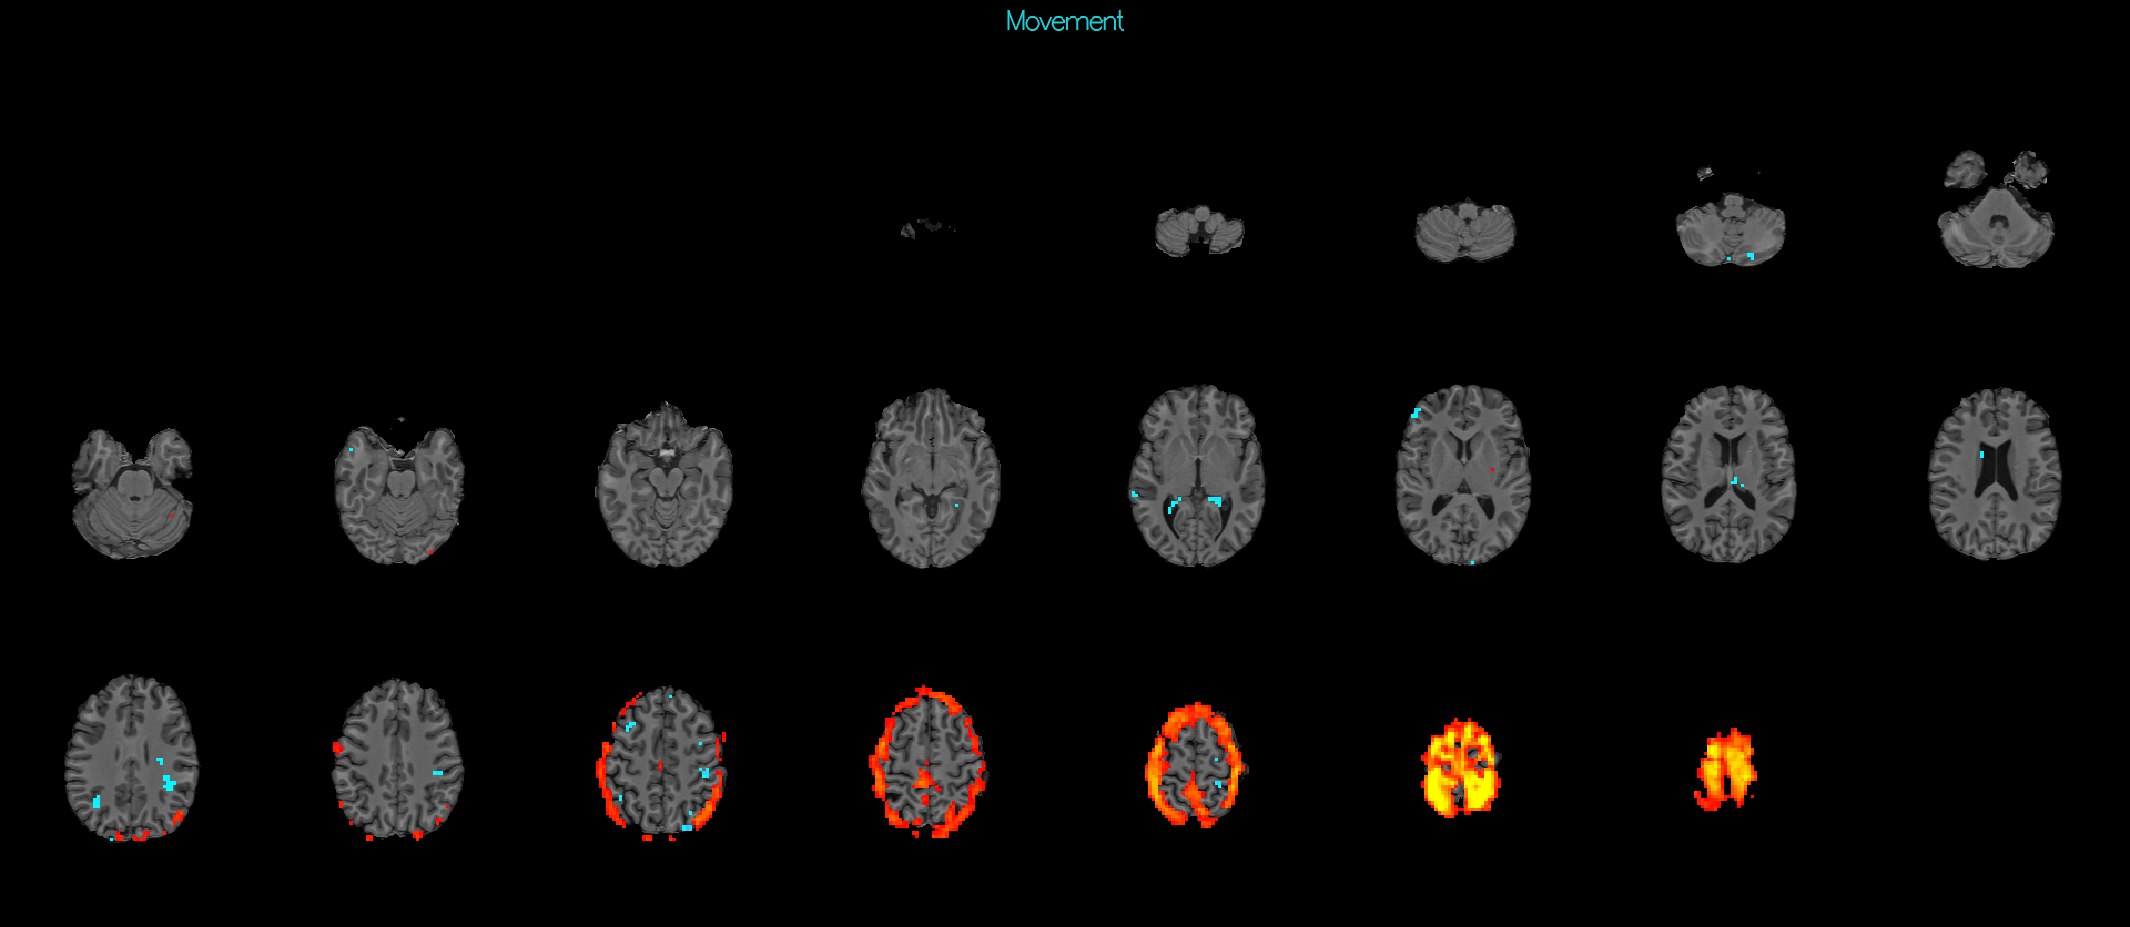
\includegraphics[width=.85\textwidth]{figures/bMethods/Movement}  
	\caption{An example component of the movement artefact. Movement noise will usually be seen as a ring or lines on the periphery of the brain. Depending on the nature of the movement causing the noise, the voxels will be located on the inside or outside of the brain.}
	\label{fig:meth:Movement} 
\end{figure}


\begin{figure}[H]                 
	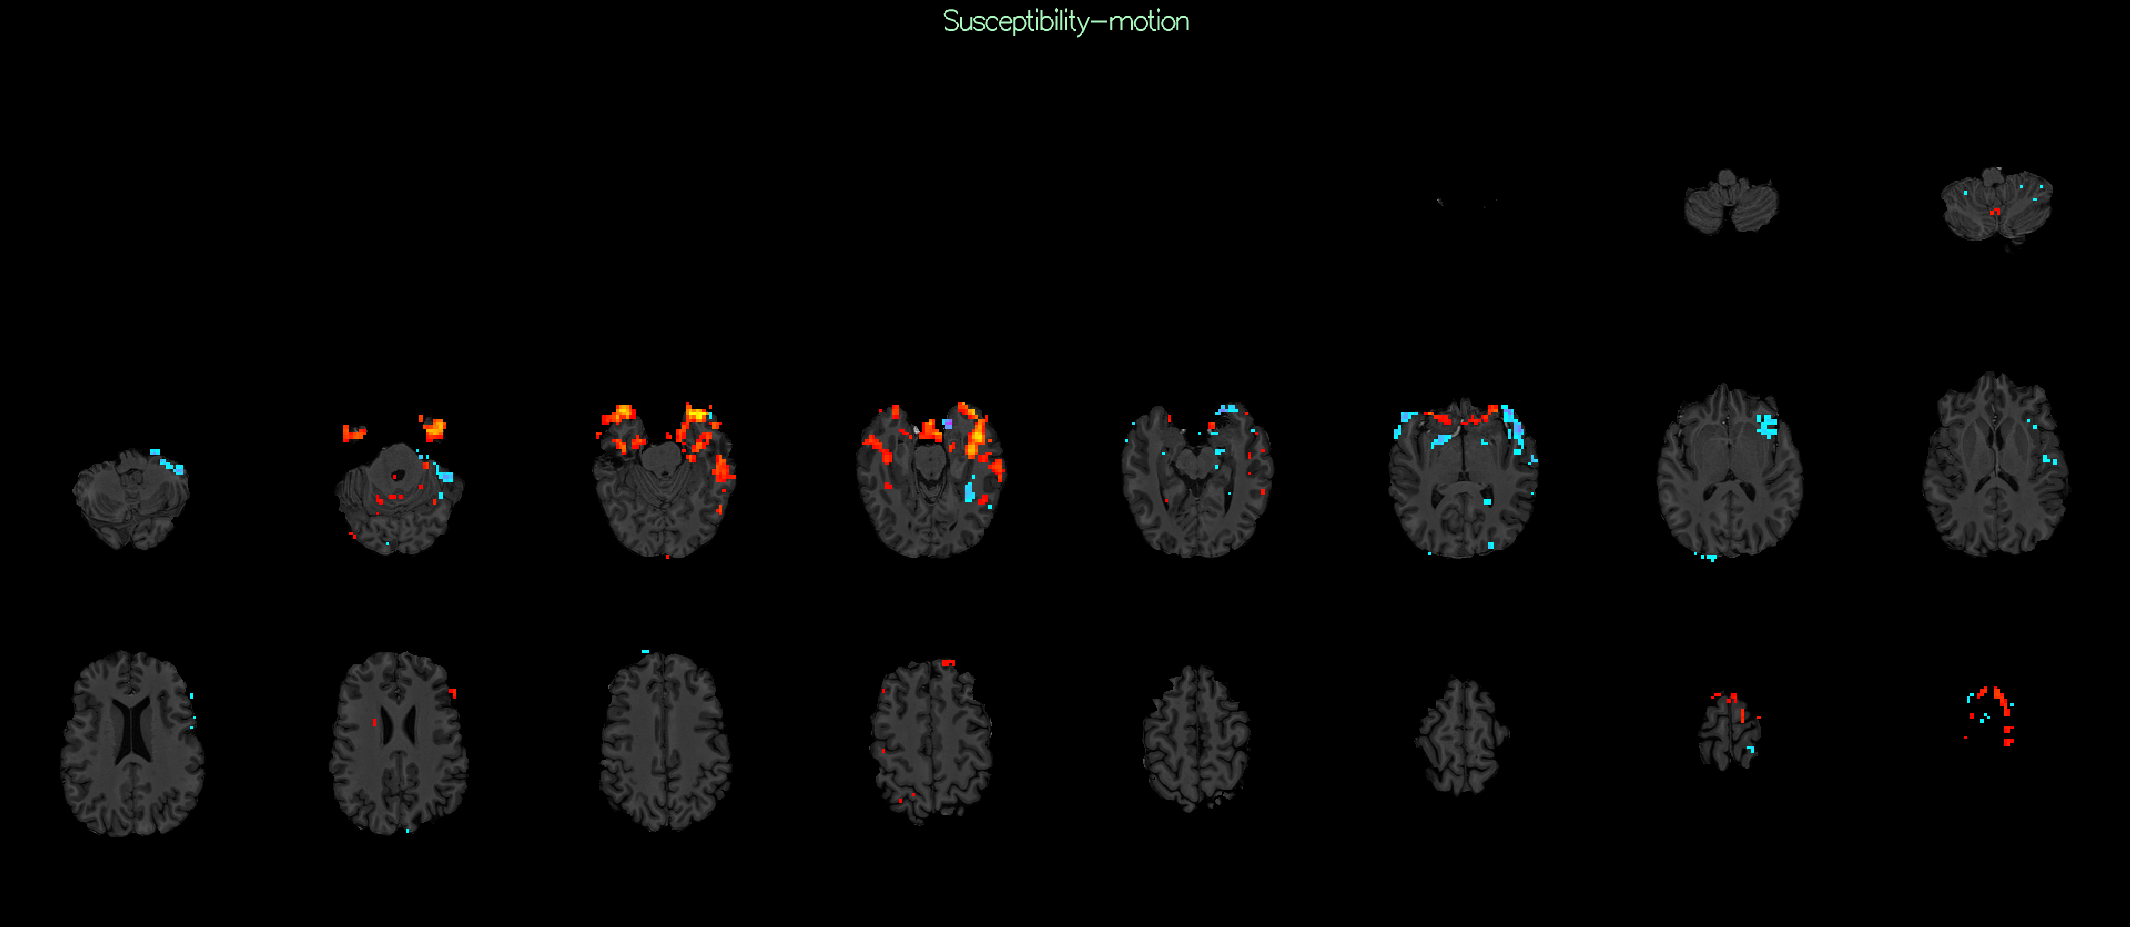
\includegraphics[width=.85\textwidth]{figures/bMethods/Susceptibility_motion}  
	\caption{An example component of the susceptibility-motion artefact. Susceptibility-motion noise is mainly due to air-tissue interfaces, and thus usually spatially expressed as a mix of activation and deactivation at the sinuses of the skull.}
	\label{fig:meth:sus} 
\end{figure}

\begin{figure}[H]                 
	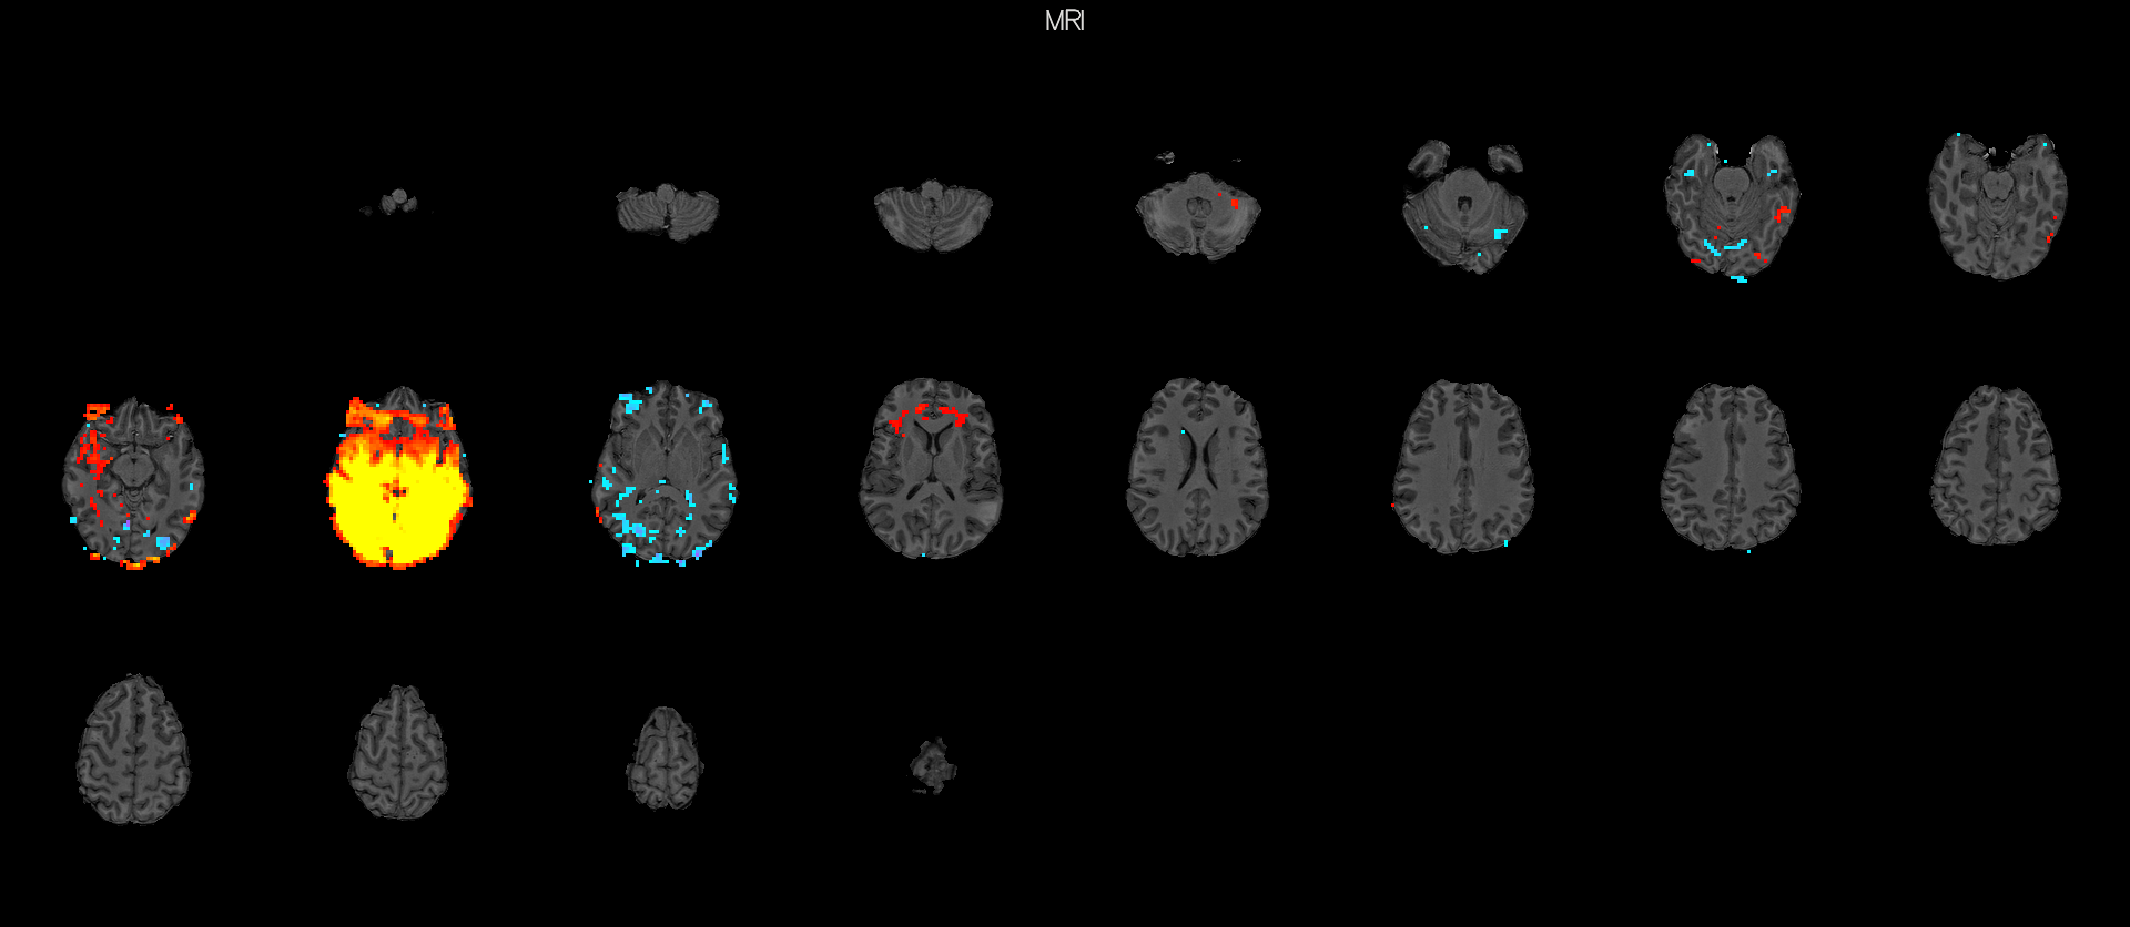
\includegraphics[width=.85\textwidth]{figures/bMethods/MRI}  
	\caption{An example component of the MRI artefact. This artefact is usually visualized as one or several fully activated or deactivated slices in separated spatial levels. In the sagittal or coronal plane, this is reflected as clear stripes in the images, which can not be explained as physiologically meaningful. Another example is slices containing large portions of alternating activation and deactivation, which too can not be physiologically explained.}
	\label{fig:meth:MRI} 
\end{figure}

\begin{figure}[H]                 
	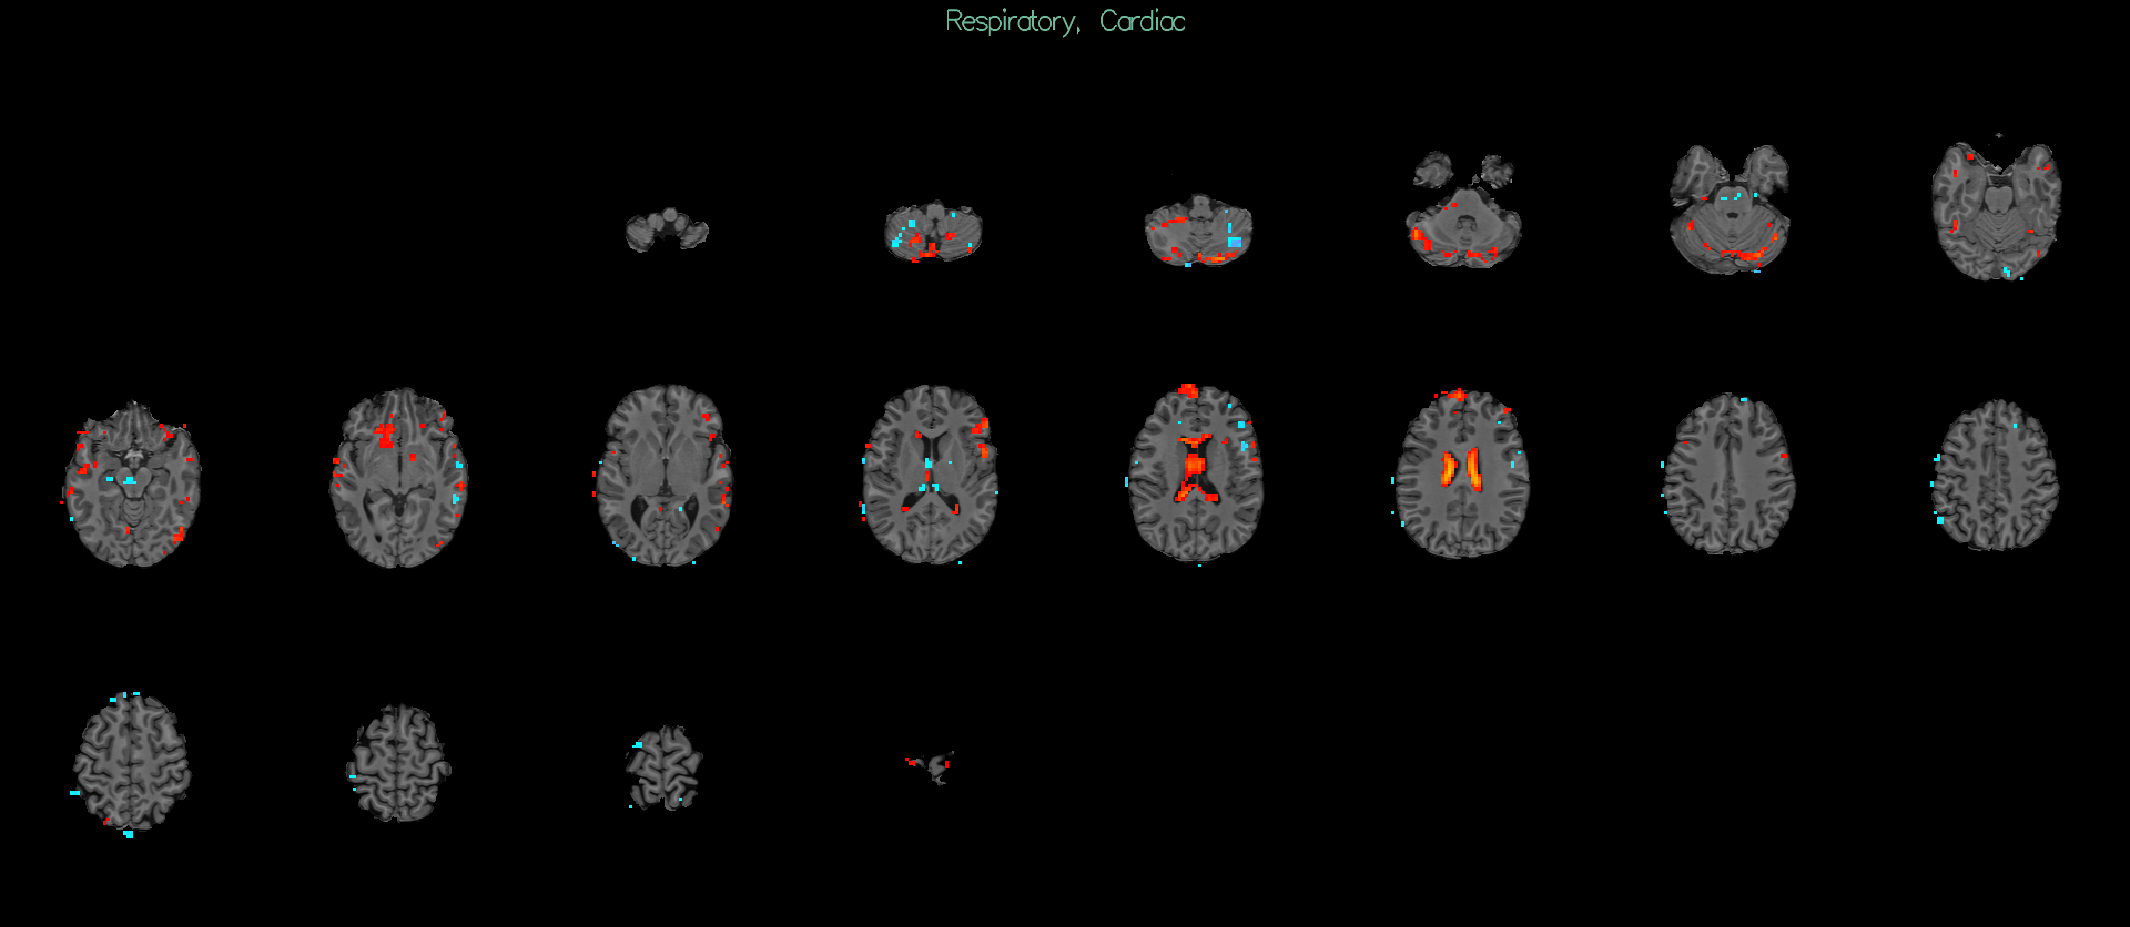
\includegraphics[width=.85\textwidth]{figures/bMethods/card_resp}  
	\caption{An example component of cardiac and respiratory artefacts. Cerebrospinal fluid pulsation is usually due to respiratory and cardiac cycles. Thus, activation of the ventricular system of the brain will be an indicator of respiratory and/or cardiac artefacts.}
	\label{fig:meth:phys} 
\end{figure}

\begin{figure}[H]                 
	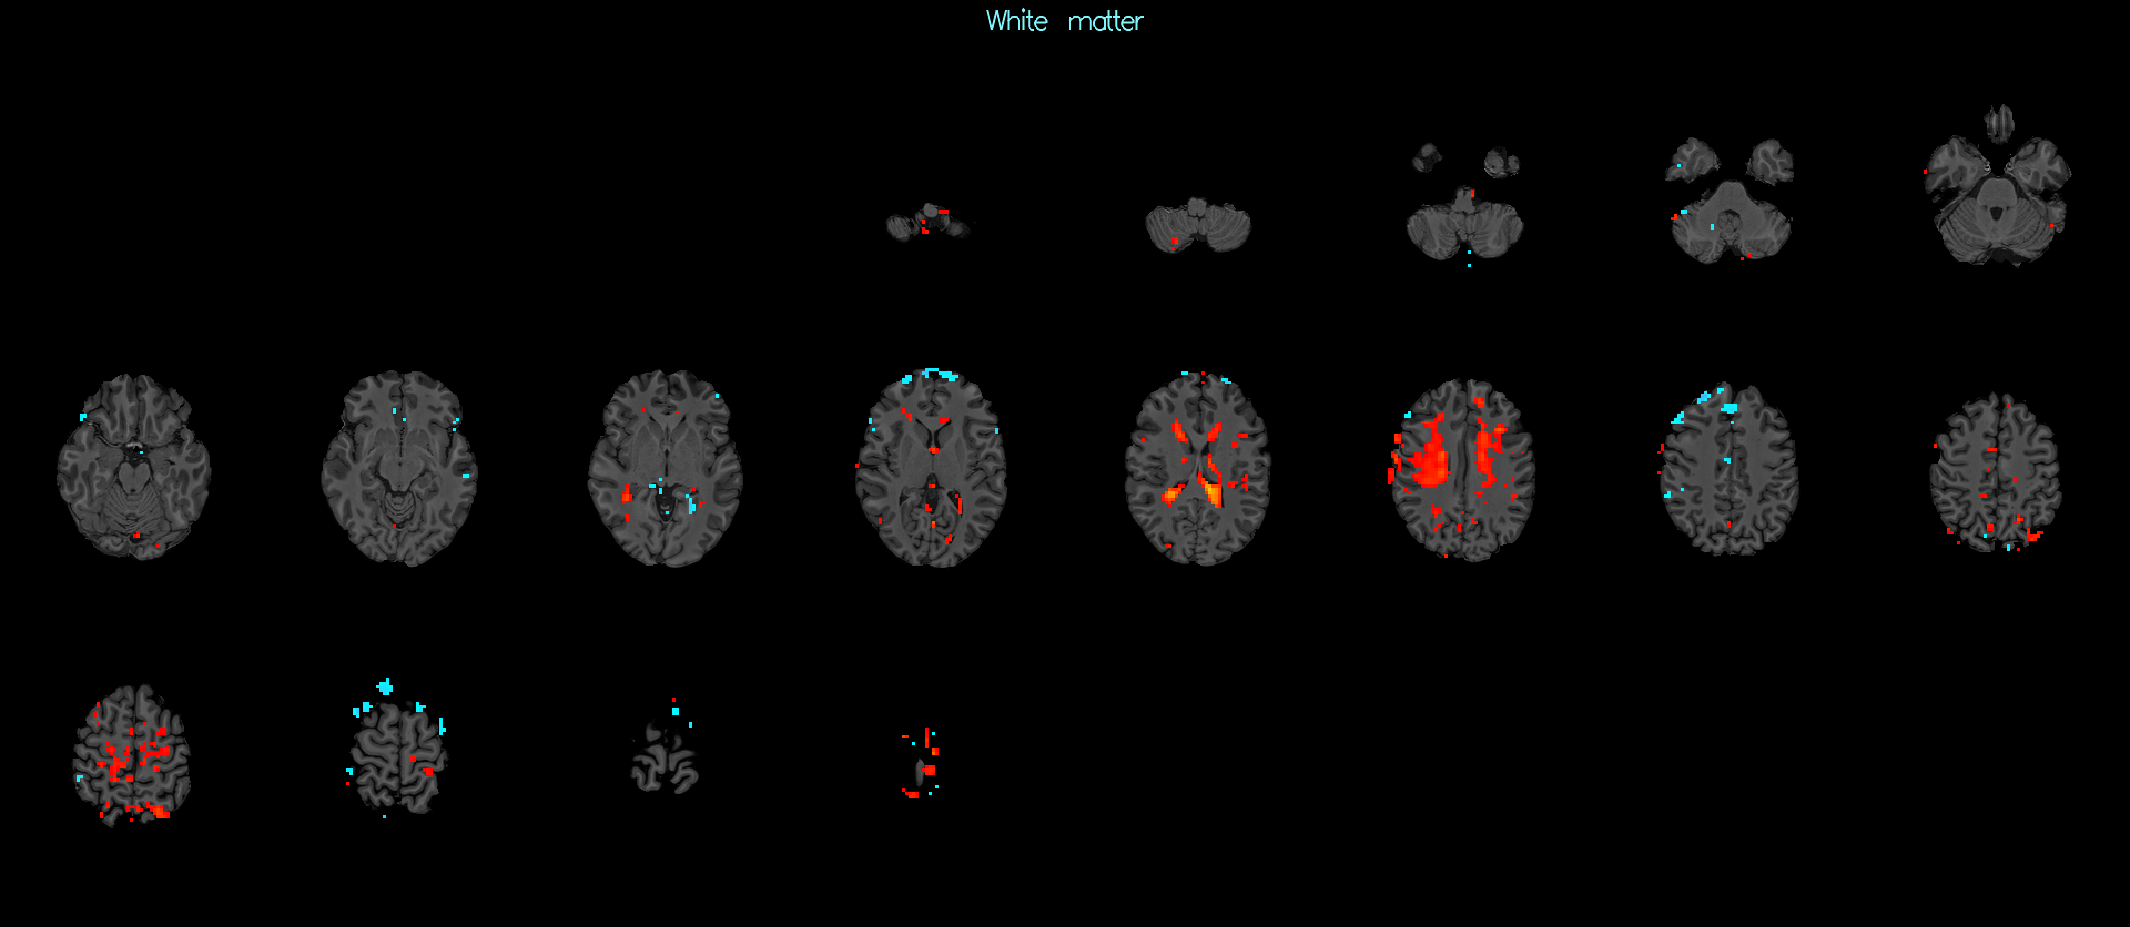
\includegraphics[width=.85\textwidth]{figures/bMethods/white_matter}  
	\caption{An example component of the white matter noise. White matter noise is visible as activation in the white matter area of the brain, while no or low activation in other regions is visible.}
	\label{fig:meth:walter_white} 
\end{figure}


\begin{figure}[H]                 
	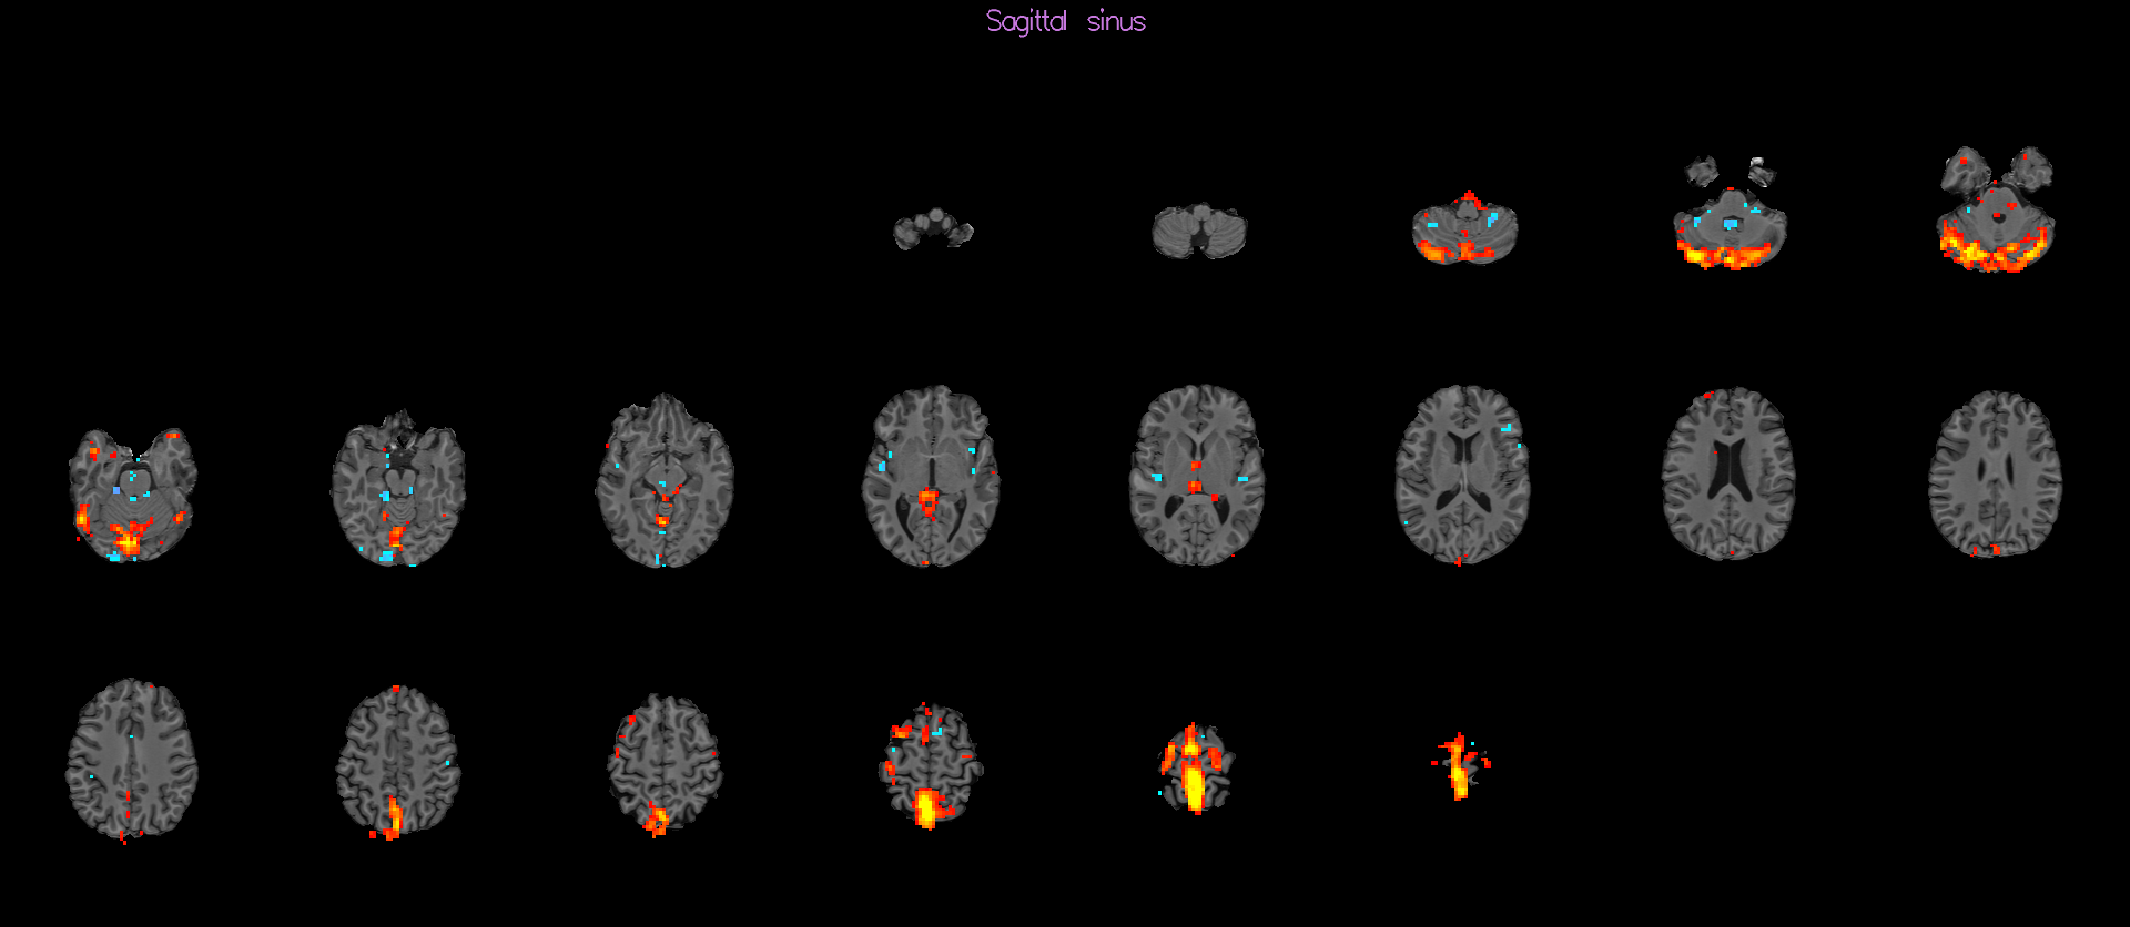
\includegraphics[width=.85\textwidth]{figures/bMethods/sag_sinus}  
	\caption{An example component of the sagittal sinus artefact. Sagittal sinus artefacts are visible as activation of the sagittal sinus veins, while no or low activation of areas of interest or noise are visible.}
	\label{fig:meth:sinus} 
\end{figure}

\begin{figure}[H]                 
	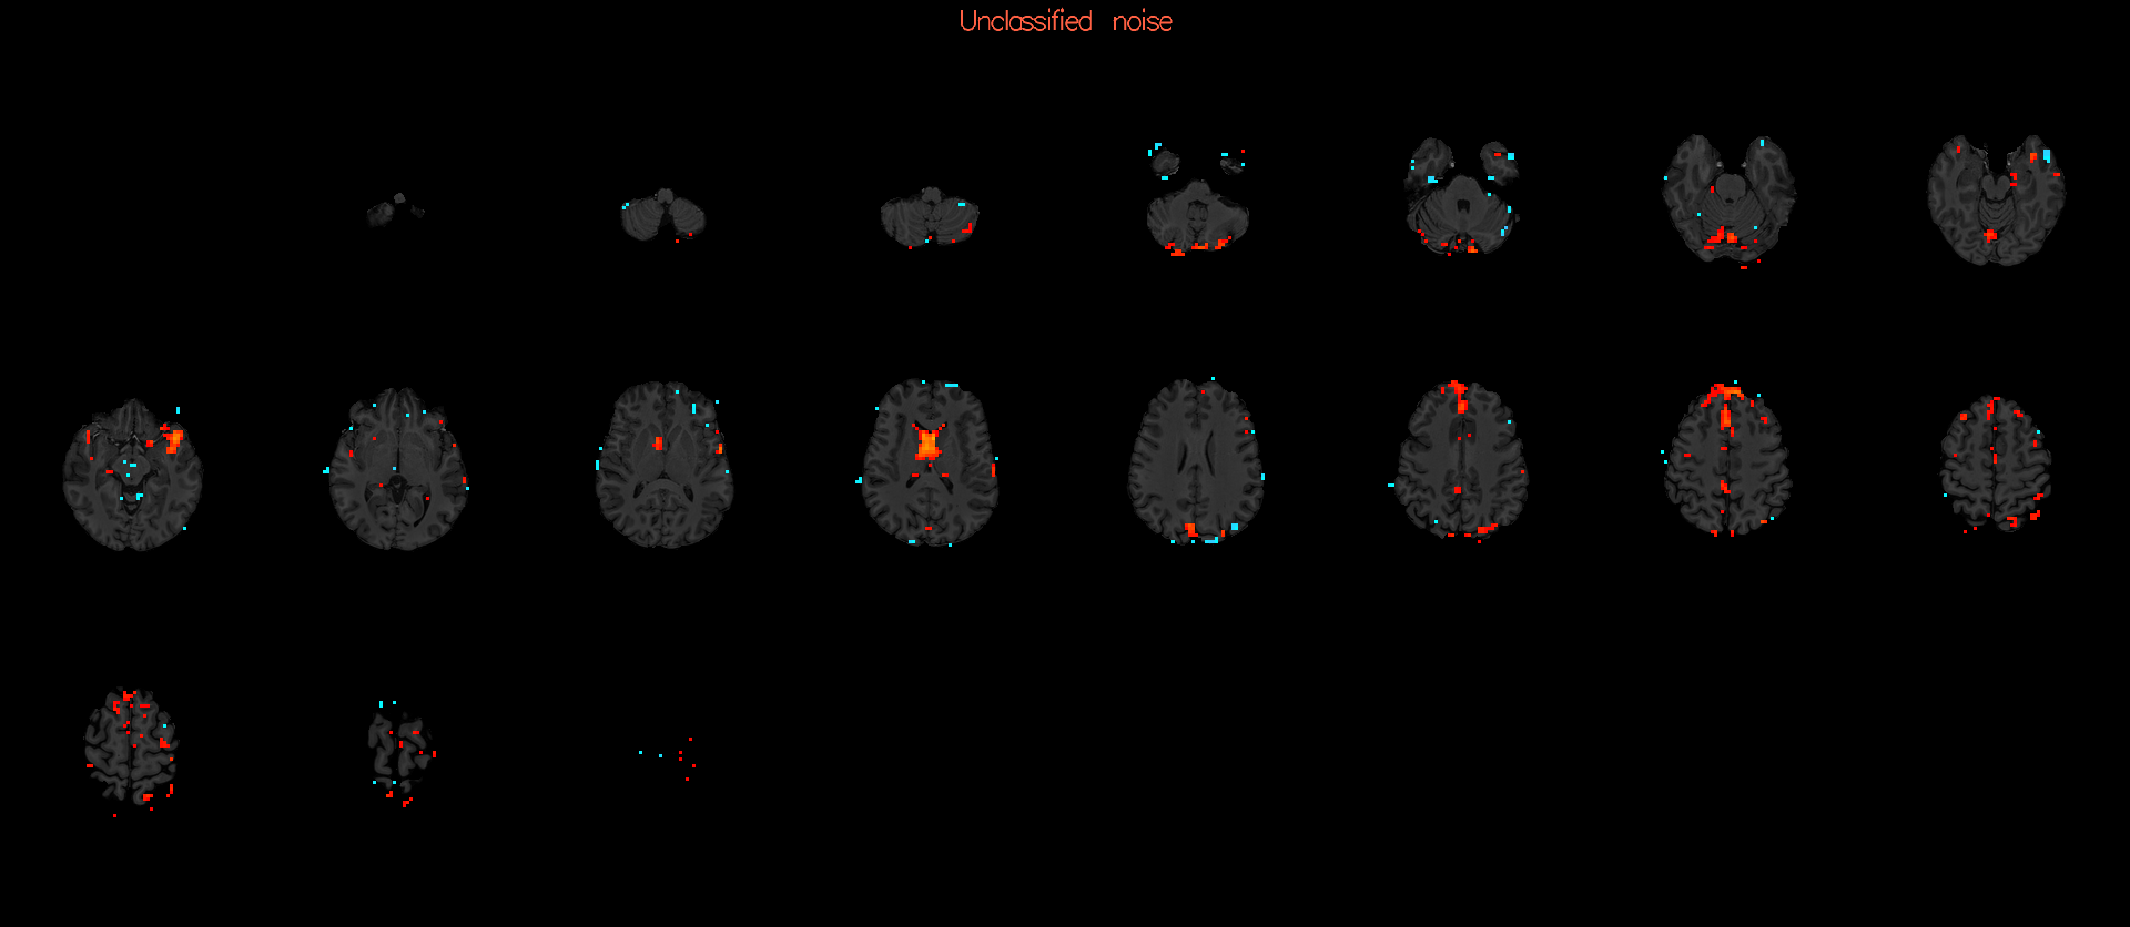
\includegraphics[width=.85\textwidth]{figures/bMethods/U_noise}  
	\caption{An example component of unclassified noise. A component was given this label when no clear noise source could be recognized and/or when the component was a mix of more than two noise sources.}
	\label{fig:meth:Unoise} 
\end{figure}


\begin{figure}[H]                 
	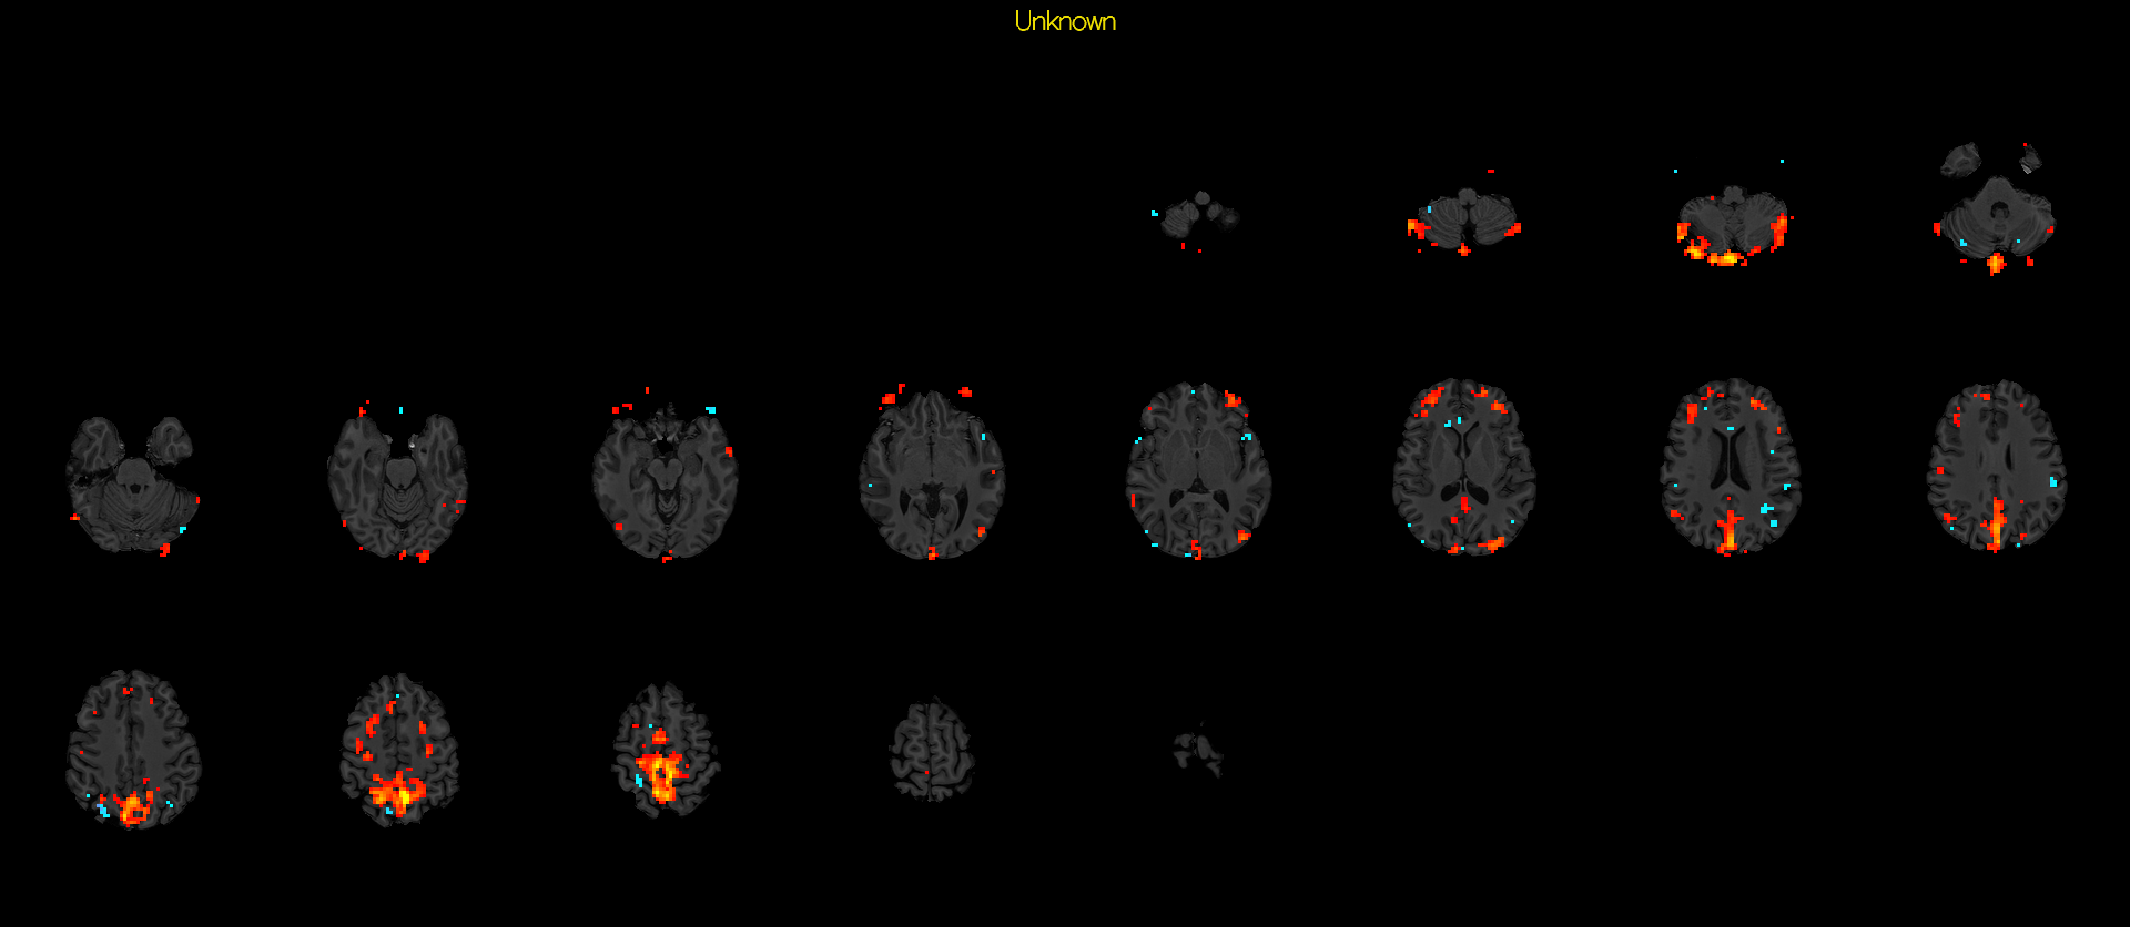
\includegraphics[width=.85\textwidth]{figures/bMethods/unknown}  
	\caption{An example component of a mix of signal of interest and noise. The signal of interest activation is either hard to localize, not seen in an expected area or the remaining spatial map is corrupted but a substantial amount of noise.}
	\label{fig:meth:unknown} 
\end{figure}

\begin{figure}[H]                 
	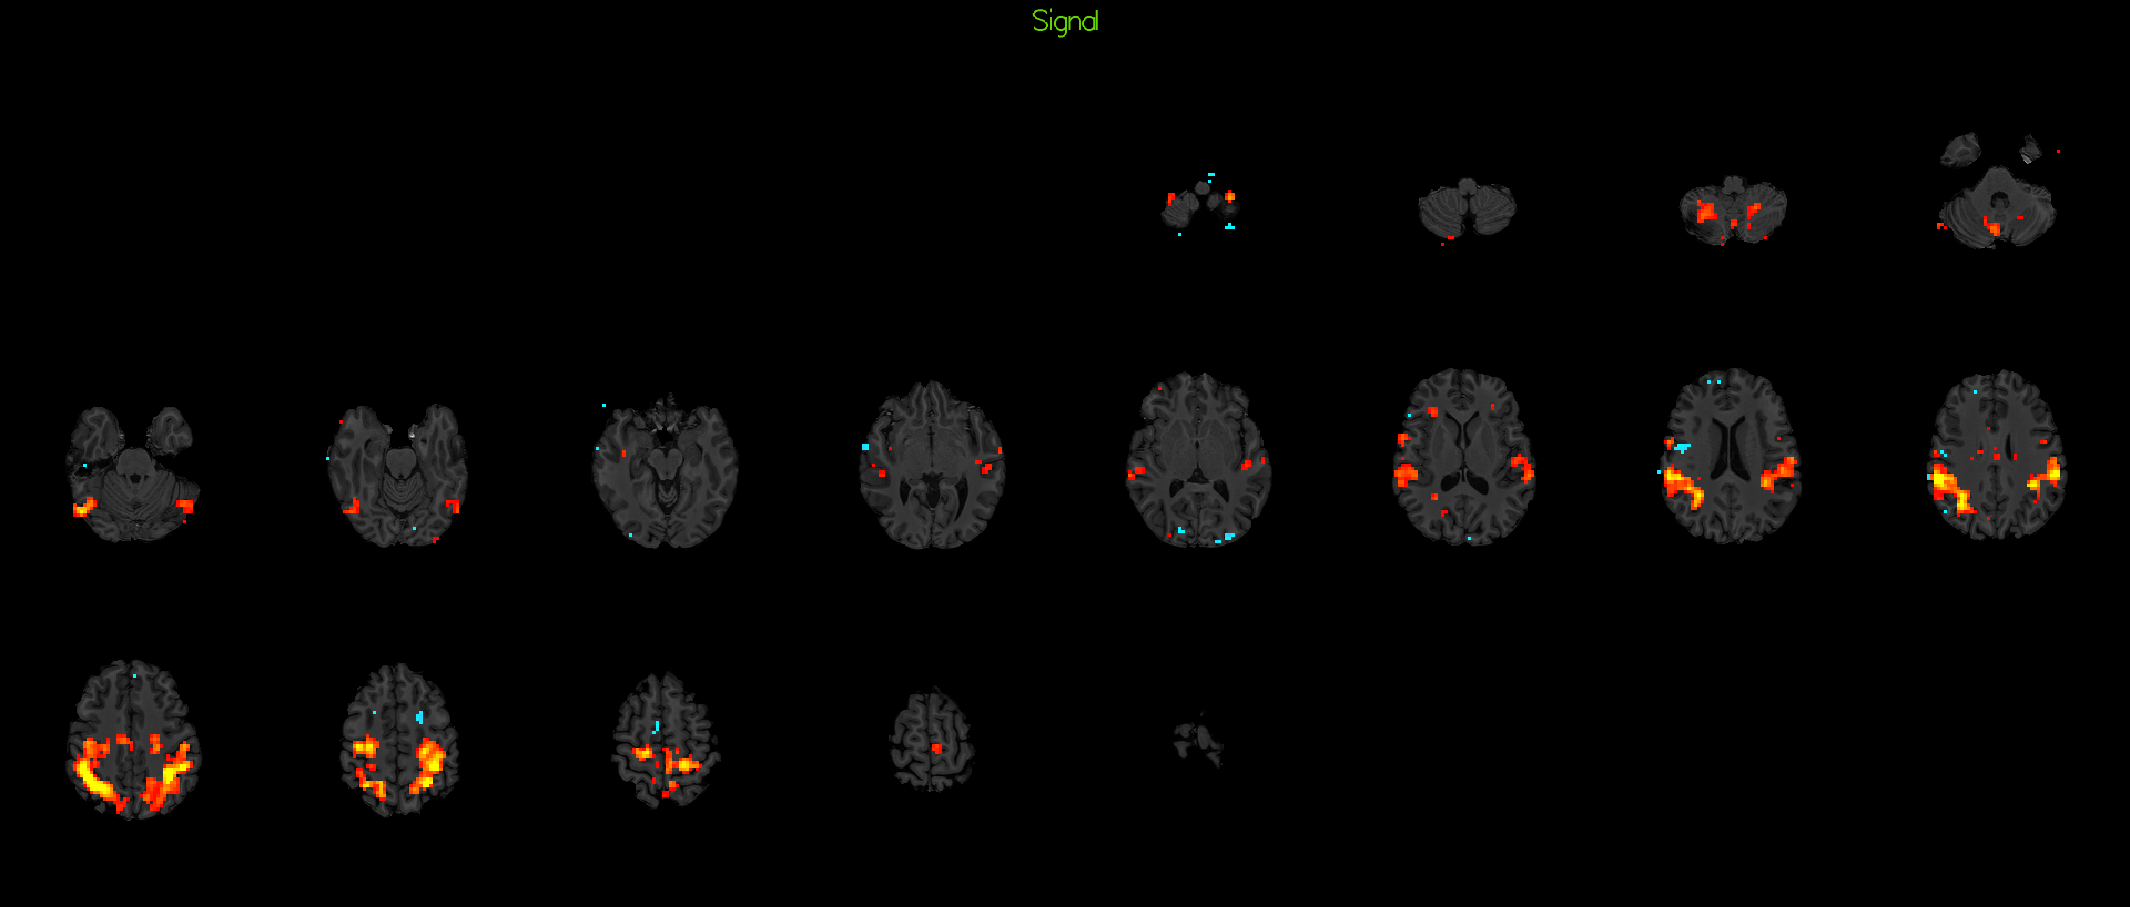
\includegraphics[width=.85\textwidth]{figures/bMethods/signal}  
	\caption{An example component of signal, which is recognizable, isolated, and not corrupted by a substantial amount of noise. In this example, the signal is characterized as a strong and fairly isolated activation mainly in the parietal lobe and temporal lobe.}
	\label{fig:meth:signal} 
\end{figure}




It should be noted that a coronal and sagittal view were additionally available, along with the time course and frequency content of each components for shaping the assessment of the labeling. The corresponding structural images were used to underlay the components to assess in which brain regions the components were located. Through the component labeling the scheme, illustrated in \figref{fig:hand_label}, was used to decide whether the component was either labeled as signal, unknown or noise. 
 
 \begin{figure}[H]                 
 	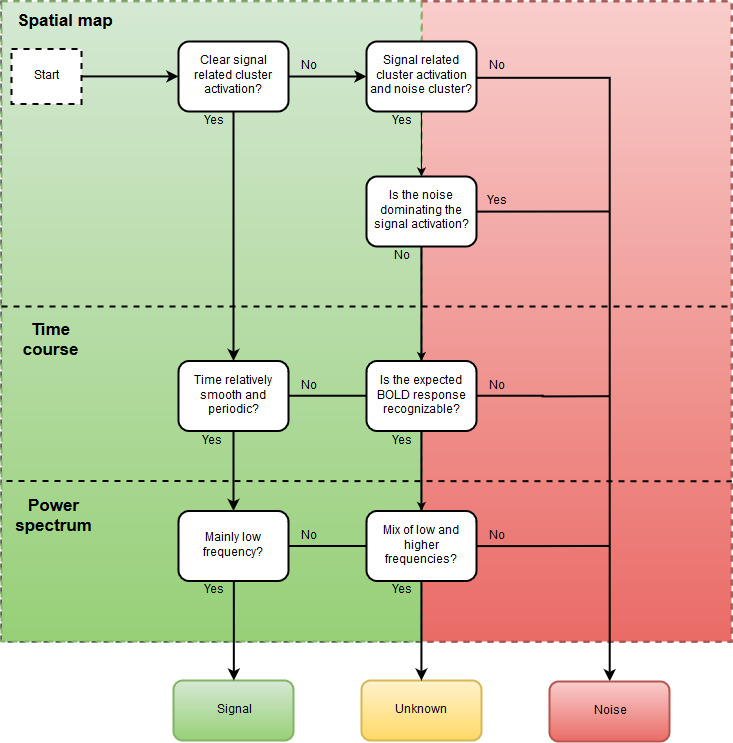
\includegraphics[width=0.85\textwidth]{figures/bMethods/Hand_labeling}  
 	\caption{A flowchart describing the assessment of a component. The component is first assessed in the spatial map, secondly the time course and lastly in the power spectrum. Note that only the assessment to either signal, unknown or noise is presented in the flowchart. When a component was found to be noise a secondary assessment into which type of noise would begin, using the information presented in \cite{Salimi-Khorshidi2014,Griffanti2017} and is therefore not accounted for in this flowchart. Illustration modified from \cite{Griffanti2017}.}
 	\label{fig:hand_label} 
 \end{figure}

\subsection{Feature extraction}
Besides training the classifier with the label of each component, it was trained with features extracted from each component. An important step in establishing a robust classification model is extracting effective features to feed the classifier. Extraction of reasonably independent features that correlate with the targeted class will establish a more robust classifier when training it. In the FIX algorithm 186 features with temporal or spatial characteristics were extracted. The first feature extracted was, however, considered of spatial-temporal origin and consisted of the number of ICs estimated by MELODIC. It would be expected that the noise present in the data would affect the number of ICs extracted. \cite{Salimi-Khorshidi2014} However, in this study the number of ICs calculated for each heat run was fixed on 25, and that feature would therefore have no influence on the expectation of a component containing noise or signal. 
The following sections aim to explain the idea behind extracting these exact temporal and spatial features and to give examples of selected features. Thus, not all 186 features will be covered in depth. For a further explanation of the features we direct the reader to the 2014 study by Salimi-Khorshidi et al. \cite{Salimi-Khorshidi2014} The result of the feature extraction from one heat run consisted of a 25 x 186 matrix - one feature value for each feature of each component.

\subsubsection{Temporal features}
\textit{Autoregressive models} Some temporal features extracted were based on autoregressive (AR) properties of the time course. It was expected that the temporal smoothness derived from AR models, could help distinguish signal from particular artefact components. For an AR(n) model, where $n$ is the order up to $n = 6$, $a_k$ denotes the AR parameters, $e_p$ denotes the variance of the residual of up to AR(6). The first AR property features derived were the slope and intercept of the straight line which explained $e_p$ as a function of $n$, where an increase in $n$ would output a better fit and thus a smaller residual variance. It was expected that an improvement in goodness of fit would decrease as more noise was present in the time course. 
The other AR features extracted were $a_1$, $a_2$, $e_1$ and $e_2$. These features encapsulated the autocorrelation estimated from the low order AR models. It was expected that components containing signal would have a higher temporal autocorrelation and lower residual variance compared to components containing noise. \\
\textit{Distribution information} It was expected that signal components would be normally distributed, while noise components would vary in how they were distributed (e.g. long-tailed distribution and multi-modal), e.g. due to sudden spikes in the time course caused by rapid movements and/or scanner artefacts. Features that gave information on distribution were therefore extracted. These included kurtosis, skewness, mean-median difference, entropy and negentropy. \\
\textit{Jump amplitudes} The extent of jumps in the amplitude of the time course is an important feature in distinguishing signal from noise. Signal components were expected to be fairly smooth, while noise components usually would contain large jump and fluctuations. To describe this characteristic features based on division calculations that include the standard deviation (std), mean or maximum of the differential of the time course and the std, mean and/or maximum of the time course were extracted. \\
\textit{Fourier transform} Taking the fast Fourier transform (fft) of the time course will capture the frequency content, which can be utilized to differentiate between signal and noise. It was expected for signal components to almost exclusively have high power amplitude in low frequencies due to the block design of the stimuli task. Noise components might on the other hand have contained frequencies of the whole spectrum. Therefore several fft-based features were extracted. Examples of features derived were the total power above 0.1, 0.15, 0.2 and 0.25 Hz respectively and the percentage of power that lied in the following intervals: 0:0.01, 0.01:0.025, 0.025:0.05, 0.05:0.1, 0.1:0.15, 0.15:0.2 and 0.2:0.25 Hz. \\
\textit{Correlation} It was expected that time courses of signal components would be strongly associated with grey matter, while noise components would correlate with time courses of white matter and CSF along with the motion correction time courses calculated in the initial preprocessing. The correlation-based features extracted were therefore based on the correlation between the component time course and reference grey matter-, white matter-, CSF-derived time courses and the motion correction time courses. The reference time courses were calculated using FSL’s tissue segmentation tool, from which grey matter, white matter and CSF masks were extracted. Each tissue type's time course was then computed as the average of the time courses that corresponded to that given tissue. \cite{Salimi-Khorshidi2014}

\subsubsection{Spatial features}
\textit{Clusters’ size and spatial distribution} The distribution of activated and deactivated cluster sizes is an important indicator of a component containing either noise or signal. It was expected that signal components contained a small number of relatively large clusters, while noise components contained a large number of small clusters. To capture this information, a list of a spatial map’s clusters $\mathbf{c}$ was formed, where only clusters of at least 5 connected activated or deactivated voxels were kept, and listed in descending order. Feature extracted to summarize $\mathbf{c}$ were: length($\mathbf{c}$), mean($\mathbf{c}$), median($\mathbf{c}$), max($\mathbf{c}$), var($\mathbf{c}$), skewness($\mathbf{c}$), kurtosis($\mathbf{c}$), $\mathbf{c}$[1], $\mathbf{c}$[2], and $\mathbf{c}$[3], where the last three features were the first to third elements of $\mathbf{c}$.\\
Looking at the distribution of clusters in individual slices can help detect scanner artefacts. $\mathbf{V}$ and $\mathbf{U}$ contained slice specific information of the ICA spatial map $\mathbf{m}$ and slice specific information of voxels above 2.5 z-score $\mathbf{m^{\tau}_{p}}$, respectively. Further features consisted of max($\mathbf{V}$) and max($\mathbf{u}$) and slices containing above 15 clusters.\\ % of the total variance of $\mathbf{V}$ and $\mathbf{u}$. Similar features examines the difference in variance explained by even and odd slices as well and the difference in variance explained by slices $[1,2,5,6,9,10, …]$ and $[3,4,7,8,11,12, …]$ for both $\mathbf{m}$ and $\mathbf{m^{\tau}_{p}}$. 
It is not very likely for signal components to have large contents of both activation and deactivation in the spatial map. For this reason features that use the mean, standard deviation and entropy of $\mathbf{m}$ to measure the amount of positive and negative voxels in the components were extracted. \\
\textit{Voxels overlaying dark/bright raw data voxels}
Signal of interest is associated with dark voxels where noise is usually found in bright voxels. The next features were based on multiplying and dividing the components’ spatial map with the mean of the corresponding preprocessed time courses, which formed two new images. It was expected that the intensity information contained information on which voxels were of interest and which were not. The features consisted of the 95th and 99th percentile of the new images. \\
\textit{Percent on brain boundary} High activation/deactivation in the spatial map that overlaps the boundary of the brain and the area outside the brain will most likely be movement related. Segmenting the brain using the FSL BET tool and subtracting this mask with and eroded version of itself will output a mask of the brain’s edge. Five masks with varying thickness were extracted. The features measured how large a percentage of activation in the components spatial maps that was embedded in the edges and how large a percentage of edges was covered by the components activation. The higher these values were, the higher probability the component was to have captured a movement artefact. \\
\textit{Mask-based features} It might be needed to use spatially-specific masks to detect certain noise sources (Sagittal sinus, CSF and White matter) more precisely. The spatial appearance of the major veins could for instance be mistaken for signal of interest and the cluster-like activation pattern may look similar to signal of interest. To detect these structures more conservatively FIX utilized three standard-space masks that consisted of three major veins. From the three masks three different masks with varying thickness were derived, due to the anatomical variability between subjects. The same features as in the brain boundary features were extracted, where these new masks were utilized instead. The same procedure was executed for grey matter. \\
\textit{Other spatial features} Other features detected spatial smoothness. Signal components were expected to have high spatial smoothness, meaning a fairly small amount of connected clusters, where noise components were expected to have a more patchy spatial map. Features that extracted spatial smoothness in millimeters and voxels counts were therefore included. Some spatial features detected striped patterns of interleaved positive and negative activation. A largely striped pattern in the spatial map could imply that a component contained noise. \cite{Salimi-Khorshidi2014}

%The derived features from one heat run from one subject consist of a 25 x 186 matrix - one feature value for each feature of each component.




\subsection{Classification algorithm}

The most important function of the classifier is to correctly separate the noise components from the signals of interest. However, it is highly probable that components do not purely contain either noise or signal, and that the characteristics of the various types of artefacts overlap. Thus, in a the context of a classification model, noise and signal are not left as two well-defined clusters in both the temporal and spatial domain, and the decision boundaries separating noise from signal will be complex. \cite{Salimi-Khorshidi2014} \\
A first step in simplifying the decision making process was to divide features into subsets, partially through a feature selection process. The reasoning for this was that some components might have more clear signal fluctuations shown only in either temporal or spatial features or other feature subsets. Let $S = S_t{\cup}S_s$ denote the full feature set, where $S_t$ and $S_s$ are the full temporal and spatial feature sets. On these subsets FIX applies feature selection based on F-scores for each feature to calculate signal-noise discrimination and logistic regression and a linear support vector machine (SVM) for ranking features. Then $S_{sel{\supset}S}$ denotes a feature subset of $S$, which contains both temporal and spatial features, denoted $S_{t-sel}$ and $S_{s-sel}$ respectively. The resulting subsets are then $S, S_t, S_s, S_{sel}, S_{t-sel}$ and $S_{s-sel}$, which were used to train the classifier (all the subsets have a column vector containing the label of each component). \\
To achieve a robust classification of components using these subsets of extracted features, there exist no ultimately best classifier. Each classifier has its weaknesses and strengths. The k-nearest neighbor algorithm (kNN) is a decent local classifier, but struggles with detecting patterns in a full dataset; SVMs is great at finding decision boundaries with maximum between cluster variance; decision trees are great at finding complex decision boundaries that can be described by a set of if-then rules. To compensate a classifier’s weakness through another’s strength, FIX employed an ensemble learning method called classifier stacking. Here the output of several single “lower level” classifiers becomes the input in a “higher-level” classifier - a fusion of different classifiers. The “lower level” classifiers consists of decision tree, kNN, SVM with radial basis function $(RBF)$ kernel $(SVM_r)$, SVM with polynomial kernel $(SVM_p)$ and linear SVM $(SVM_l)$. Another reasoning for using these specific classifiers was that they could produce a probability output between 0 and 1, where 0 denoted perfect noise and 1 denoted perfect signal. Each of the six subsets were fed to each of the 5 classifiers, thus producing 30 probability values (5 x 6 matrix) between 0 and 1 which function as input to the “higher level” classifier. The “higher level” classifier consists of multiple classifiers: $SVM_l$, $SVM_r$, random forest, and conditional-inference tree, that learns how to best combine the inputs. \\
Thus, training this ensemble learner algorithm consisted of selecting the data subsets, training the “lower-level” level classifiers, whose output was the input of the “higher level” classifier, whose output was the probability of a component being noise or signal. A graphical illustration of the classifier design can be seen in \figref{fig:classifier}. \fxnote{(elaborate on the structure of the higher level classifier.)}

\begin{figure}[H]                 
	\includegraphics[width=.95\textwidth]{figures/bMethods/classifier}  
	\caption{An illustration of the classifier design, where the six feature subsets can be seen feed to five different classifiers in the lower level classifier. The output from each of 30 classifiers was a 5 $\times$ 6 probability matrix, containing the probability for each. This matrix was then feed to the higher level classifier consisting of four classifiers, deciding the final component label. Modified from \cite{Salimi-Khorshidi2014}.}
	\label{fig:classifier} 
\end{figure}

\subsection{Estimating component label threshold}
The classifier in FIX required setting a threshold on how soft or aggressive the classifier should be at including potentially noisy signal components. This threshold scale varied from 1-100, where 1 was the most soft, meaning that almost no components containing some portion of signal of interest are labeled as noise. \\
To be able to perform a quantitative evaluation of which threshold to choose, the FIX software provided the leave-one-out(LOO) classification option. On a data set containing \textit{n} outputs (e.g. one for each heat run per subject), a cross-validation was performed, where each fold uses a \textit{n-1} data set for training and tests the obtained decision boundary on the data set left out. This LOO was carried out using the following thresholds: 1, 2, 5, 10, 20, 30, 40, 50. For each heat run and each threshold the following was additionally calculated: true-positive ratio (TPR), true-negative ratio (TNR) and a weighted ratio (WR), $\frac{3*TPR+TNR}{4}$, which favored the TPR. Summarizing these values as the mean across all heat runs yielded an accuracy matrix, from which a decision on which threshold to choose could be based upon. \\
After performing the LOO classification with the training data from this project, it was observed that a TPR of NaN for all thresholds was calculated for two of the heat runs; possibly due to the heat runs not containing any signal components. This resulted in the mean TPR and the WR being NaN for all thresholds. These two heat runs were therefore excluded from the project. The resultant accuracy matrix of the LOO classification can be seen in \tabref{tab:decisionmatrix}.

\begin{table}[H] 
	\caption{Accuracy matix from the LOO classifier. TPR denotes the mean percentage of true signals correctly classified. TNR denotes the mean percentage of true noise correctly classified. WR is a weighted ratio that favors TPR. The more the threshold increases the lower the TPR and the higher the TNR.}\label{tab:decisionmatrix}
	\begin{tabular}{l|llllllll}
		Threshold:                              & 1    & 2    & 5    & 10   & 20   & 30   & 40   & 50   \\ \hline
		TPR:                                    & 99.1 & 98.6 & 98.4 & 97.3 & 96.3 & 94.3 & 92.4 & 91.4 \\ %\cline{1-1}
		TNR:                                    & 78.1 & 80.9 & 85.5 & 90.2 & 93.7 & 95.5 & 96.6 & 97.7 \\ %\cline{1-1}
		WR: & 93.9 & 94.2 & 95.2 & 95.5 & 95.7 & 94.6 & 93.4 & 93.0
	\end{tabular}
\end{table}


For this project it was important that much signal was kept, while not including too much noise. This demand was well summarized by the WR. Thus, the threshold with the highest WR (20) was initially chosen. However, it was recommended by the FIX developers to validate the most prefered thresholds quantitatively, before making a final decision. The test data set was therefore run on the trained classifier using the thresholds with a WR above 95 \% (5, 10 and 20). Checking the classified labels on three subjects per threshold, left the initial decision on choosing a threshold of 20 to stand.


\part{Synthesis}


	
\urlstyle{same}
\printbibliography
\clearpage



\cleardoublepage
% BILAG
\begin{appendices}
	\chapter{Appendices}
\section{MRI physics} \label{sec:physics}

Magnetic Resonance Imaging (MRI) is a non-invasive imaging technology, which does not involve potentially damaging ionizing radiation as in other scanners, eg. CT and X-ray. MRI is especially suited for representing soft tissue portions of the body, which makes it a widely used technology in brain imaging, both for clinical and research purposes, as it can depict the anatomical structure at a millimeter resolution. This section will provide information on the physics behind MRI and which physiological properties that can be exploited to create an image of the body.
 
Magnetic resonance imaging (MRI) is founded on the principle of nuclear magnetic resonance (NMR), which exploits the magnetic properties of the hydrogen nucleus that contains a single proton. The proton is not static, but rotates around its own axis. As the proton is positively charged it creates a magnetic moment in the direction described by the thumb rule, and can interact with an external magnetic field. The human body consists of approximately 10\% hydrogen atoms, but as the hydrogen nuclei spins are randomly orientated, the net magnetic moment equals zero, as the nuclei cancel each other out. Placing the body in a strong magnetic field will align the nuclei. A property of the hydrogen nucleus is its quantum spin rate, which can either be $ \frac{1}{2}$ or $- \frac{1}{2}$ either in the direction or the opposite direction of the main magnetic field. Most will align in the direction of the magnetic field, while the rest align in the opposite direction, possibly as a result of heat radiation absorbed by the nuclei. The direction of the nucleus is determined by its energy level, leaving the former in a low energy state and the latter in a high energy state. The nuclei do not simply point in the direction or opposite the direction of the magnetic field, but precess. \cite{Bharath2008} The rate of precession can be calculated by the Lamour frequency:
\begin{equation} \label{eq:lamour}
f=y*B_0
\end{equation} 
$f$ is precession frequency, $y$ is gyroscopic ratio and $B_0$ is magnetic field strength. The equation states that the precession frequency is proportional to the strength of the magnetic field. After canceling out all opposing precessing nuclei, the net magnetization, or longitudinal magnetization, will point in the direction of the external magnetic field. However, the longitudinal magnetization can not be detected directly as it points in the direction of the strong external magnetic field. Additional techniques are therefore used in NMR, to facilitate a detectable signal. \cite{Bharath2008} A depiction of how the nucleus precessing can either align along or opposite to the magnetic field depending on its energy state, can be found in \figref{fig:back:nucleus_precess}.  \\

\begin{figure}[H]                 
	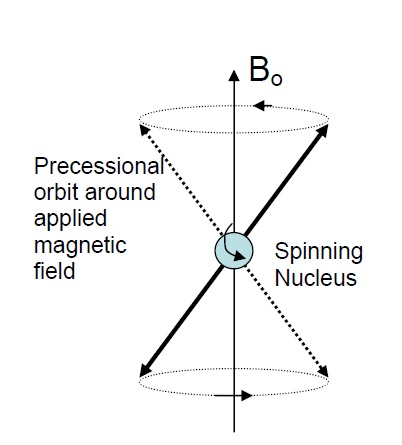
\includegraphics[width=.375\textwidth]{figures/aBackground/nucleus_precess}  
	\caption{The figure illustrates how the nucleus precess and spin in relation to the applied magnetic field $B_0$ surrounding it. The vectors, indicating the precessing, can go opposite or along the magnetic field depending on the nucleus energy state. \cite{Edwards}}
	\label{fig:back:nucleus_precess} 
\end{figure}  
A radio frequency pulse (RF pulse) tuned to the precession of the nuclei is transmitted in the vicinity of the nuclei. The RF pulse is absorbed by the nuclei and more, favorably half of the targeted nuclei population, will enter the high energy state, leaving the longitudinal magnetization to equal zero. The number of nuclei that flip is determined by the amount of energy the RF pulse injects, and the nuclei only exchange energy efficiently if the frequency of the energy from the RF pulse matches the precession rate. The RF pulse furthermore shifts the precession of the nuclei into same phase angle, which creates resonance, and a net magnetization pointing 90$^\circ$ to the longitudinal magnetization. This magnetization is called the transverse magnetization. The coherent nuclei produce a radio signal, or free induction decay signal (FID signal), that can be detected by a radio antenna. 
After the RF pulse is removed, the nuclei will relax into baseline state. Firstly, the spins of the nuclei will repel each other, as they are positively charged, and thus shift phase. The net magnetization will return to zero. This relaxation is called $T_2$ or “spin-spin” relaxation, as the energy exchange between the nucleus spins is causing the relaxation. An illustration of the $T_2$ relaxation can be seen in \figref{fig:back:T2_relax}. 

\begin{figure}[H]                 
	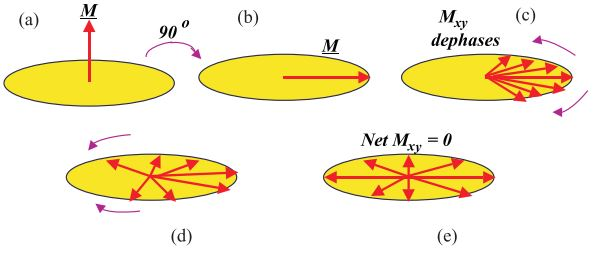
\includegraphics[width=.76\textwidth]{figures/aBackground/T2_relax}  
	\caption{An illustration of the $T_2$ relaxation. Before the RF pulse is emitted the majority of the nuclei are precessing out of phase in the low energy state and the net magnetization is pointing in the direction of the longitudinal magnetization, $(a)$. The nuclei absorb the RF pulse, the magnetization shifts $90 \degree$ and the nuclei precess in phase, which leaves a high transverse magnetization and FID-signal, $(b)$. Due to interaction between the nuclei spins, the nuclei gradually dephase, until the net magnetization is 0, which is referred to as $T_2$ relaxation. \cite{Bharath2008}}
	\label{fig:back:T2_relax} 
\end{figure}

A second relaxation appears as the high energy nuclei returns to the low energy state. The energy that was previously absorbed by the nuclei is dissipated in to the surrounding lattice in the form of heat. During this relaxation the longitudinal magnetization is regrown. This relaxation is called $T_1$ or “spin-lattice” relaxation, as the spins transfer energy to the surrounding lattice. \cite{Bharath2008}
The hydrogen nuclei are located in different local environments in the body. Some are for instance associated with free-floating water molecules, while others are associated with structural and storage molecules such as proteins and lipids, and thus more fixed in position. The nuclei have different $T_1$ and $T_2$ relaxation characteristics, depending on the local environment or tissue they are associated with. This can be accentuated and measured in NMR. \cite{Bharath2008} \\
The chosen pulse sequence is key to how the tissue will be portrayed in an image, and is described by the $T_{echo}$, time before the FID signal is measured, and $T_{rep}$, time before a new RF pulse is applied. In a case of nuclei associated with lipids and water molecules, the nuclei in lipids are fixed and will have a fast $T_1$ relaxation after exposure to a RF pulse. Meanwhile the nuclei in the water molecules will maintain being in a synchronized phase. At $T_{echo}$, the nuclei associated with the lipids will have a low amplitude FID signal, as the transverse magnetization is weak, and the nuclei associated with the water molecules will have a high amplitude FID signal, as the transverse magnetization is strong. The water molecules will be assigned a white color on a greyscale image and the lipids as dark grey/black. In this case there is a long $T_{echo}$ and a long $T_{rep}$, and is referred to as $T_2$-weighted MRI A commonly used $T_2$ pulse sequence is the spin echo (SE). Due to magnetic field inhomogenities the nuclei dephase more rapidly. Applying a second RF pulse of 180\degree after the nuclei have dephased, the nuclei will rephase. Again the constrast in the image is expressed as a result of the relaxation time of the nuclei, which is depends on the surrounding environment. . \cite{Bharath2008} \\
\setlength{\parindent}{0.2cm} In case of $T_1$-weighted MRI, the $T_{echo}$ and $T_{rep}$ are short. As in $T_2$-weighted MRI a RF pulse is applied and the nuclei associated with lipids will quickly return to baseline state and the water molecule nuclei will remain a strong transverse magnetization. At this time point a second RF pulse will be induced, referring to the short $T_{rep}$. Now the lipid nuclei will return to a strong transverse magnetization state and excite a high FID signal. More low energy state nuclei of the water molecules will absorb the RF pulse and shift to a high energy state, leaving a majority of nuclei in a high energy state. The water molecule nuclei now has a weak transverse magnetization and 180 degrees longitudinal magnetization, thus producing a low-amplitude FID signal. A short $T_{echo}$ after the second RF pulse then shows lipids as white and the water molecules as dark grey/black in a greyscale image. \cite{Bharath2008} \\
$T_2$ relaxation was defined as dephasing due to energy exchange between nuclei. In practice the $T_2$ relaxation time happens much faster than would be predicted by these natural atomic interactions. Another factor in the dephasing of nuclei is inhomogeneities in the magnetic field. This observed $T_2$ relaxation is referred to as $T_{2}^*$ relaxation. In a $T_{2}^*$ -weighted MRI, a gradient echo (GRE) is used instead of a SE. In a GRE pulse sequence only one RF pulse is emitted with a low flip angle, and the echo time is therefore usually shorter. A gradient is applied after the initiating RF pulse, which enhances the dephasing. When the net magnetization is zero a rephasing gradient with opposite polarity of the dephasing gradient is turned on, which reverses the phase shift. A FID-signal is produced as a GRE. The gradient only reverses the phase shifts that have been affected by the gradient itself, and not those affected by magnetic field inhomogeneities. Contrast in tissues is therefore not decided through natural $T_2$ relaxation but by $T_{2}^*$. Thus, $T_{2}^*$ -weighted MRI only works well in scanners that do not lack magnetic field homogeneity. Due to the fast acquisition time $T_{2}^*$ -weighted MRI is widely used in functional MRI to image brain activity.  \cite{Chavhan2009}  


\section{MR image reconstruction}

Different pulse sequences and certain physiological properties that can be exploited with certain pulse sequences, have been laid out in the previous sections. This section aims to describe how the corresponding echo signals are reconstructed as a MR image.

Following the Lamour frequency \eqref{eq:lamour}, the main magnetic field causes all hydrogen nuclei to precess with the same frequency. Without any specification of spatial localization a MRI of a human body would consist of a single number. To prevent this, separate coils in the x, y and z directions are introduced. These coils can be adjusted in position, and thus produce gradient magnetic fields with a varying strength depending on position. According to the Lamour frequency the nuclei will precess with different frequencies when in a magnetic field with varying strength. The gradients can be turned on in combination to create any direction in space. These varying frequencies can be exploited to separate parts of the anatomy and ultimately illustrate a desired area. As mentioned, the nuclei only exchange energy efficiently if the frequency of energy, or RF pulse, matches the precession rate. Thus, by altering the magnetic field along the body in one direction, z-direction for the sake of the example, the nuclei will have slightly different precession rates, and the RF pulse will only efficiently affect a desired slice of the nuclei.
The nuclei of that slice now precess at the same rate. To get an image with a spatial resolution, the voxels that make out the image needs to be discriminated between. By turning on the gradient of the x-direction the lines in the y-direction are now encoded with a particular frequency. This gradient functions as a frequency encoding gradient, and is illustrated in \figref{fig:back:gradient}. \cite{Bharath2008} \\
 \begin{figure}[H]                 
	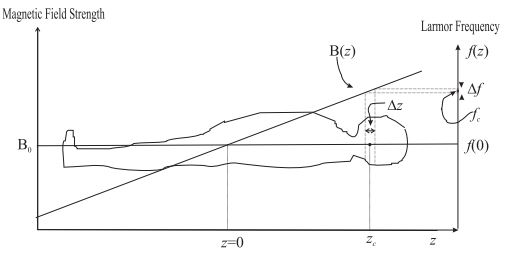
\includegraphics[width=.7\textwidth]{figures/aBackground/gradient}  
	\caption{The position of the slice is specified through the direction of the frequency encoding gradient ($B(z)$) and though the central frequency of the emitted RF pulse ($f_c$). The thickness of the slice is dependent on the steepness slope of $B(z)$, and on the bandwith of the emitted RF pulse $(\delta f)$. \cite{Bharath2008}}
	\label{fig:back:gradient} 
\end{figure}
Turning the y-gradient on and quickly off, will de-phase the nuclei while still remaining the same frequency as before. This gradient functions as a phase encoding gradient. When comparing two locations approximately one voxel apart in the x-direction, then based on the amount of gradient strength difference, there will be a certain amount of change in phase between the spins spread across that distance. The farther away from isocenter, where the magnetic field strength is $B_0$, the higher the change in phase will be. This notion is used to assign the correct spatial location of each voxel, when reconstructing the FID signals into an image. This phase encoding procedure is done in different gradient strengths in iterations to assign unique phases to the nuclei in the both directions. One iteration of a certain strength of the phase encoding gradient followed by a measurement is performed at a time. The only change per iteration is the phase encoding gradient strength. These iterations are then series of measurements acquired at different points in time, where each entry of the slice then represent a certain signal intensity. This time domain measurement is referred to at the raw data. \cite{Bharath2008}\\
The next step is to Fourier Transform (FT) the raw data, which will yield frequency information to the acquired signal intensities. This step gives a summation of the signal intensities at the different frequencies produced by the frequency encoding gradient. This is called the k-space, as the k-numbers of a signal describes its relative orientation and frequency. The k-space image contains the contrast in the center and the resolution in the periphery, as there is low or no phase encoding at the center and increasing towards the periphery, giving more brightness in the center and dimmer tones in the periphery. To allocate the voxels in correct spatial localization an inverse 2D discrete FT is performed on the k-space image. This provides the desired image of the anatomy slice. \cite{Bharath2008} \Figref{fig:back:kspace} shows the acquired signal in k-space and the reconstructed image after the Fourier Transform. 

\begin{figure}[H]                 
	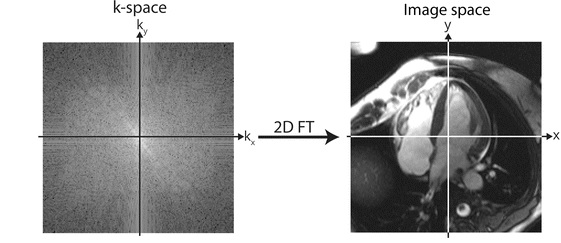
\includegraphics[width=.8\textwidth]{figures/aBackground/k_space}  
	\caption{A depiction of the acquired signal represented in k-space and the resulting reconstructed image after the inverse 2D Fourier Transform \cite{Syed2015}.}
	\label{fig:back:kspace} 
\end{figure}
\section{Stimuli Design} \label{sec:Stim}

The following section will describe different standards of designing experiments, where the impact of a given stimuli is used to assess the subsequent brain activation. The impact of stimuli on the hemodynamic response and how it is transformed into the hemodynamic response function (HRF) used analysis will be further explained. \\
In order to accomplish a well designed experiment, the researcher must consider the multiple types of stimuli delivered, including the form and duration of these. The researcher must be aware of the timing of events in the scanning session and any responses provoked. Additionally, the researcher should have general knowledge of where in the brain activation is seen and how the hemodynamic response will be presented. \cite{Moayedi2018} \\
Doing cognitive experiments using fMRI, two main design types are utilized, by either using a block- or event-related design. Event-related design is inducing a series of very short lasting stimuli used to investigate single hemodynamic response. A characteristic of this method is that it permits the possibility of increasing and decreasing the interval between stimuli. Thereby the theoretical likelihood of subject confounds should be reduced as the interval would not become predictable. Event-related stimuli design further allows more temporals characteristics to be inspected, compared to a block design. Characteristics could be hemodynamic response in duration and amplitude. \cite{Chee2003}  \\
Block design works by performing a series of less but longer stimuli. Block designs are ideal for experiments involving detection of small differences in BOLD signal across various test conditions where its statistical power is superior. Furthermore, if there is artifacts present they are more easily detected in the signal time course, because of the signals temporal structure. A block design is easier to design than an event-related, as randomization of intervals of stimuli is not required. The design instead focuses on the total number of stimuli used, block length, inter stimulus interval, block length and TR. An illustration of both design types can be found in \figref{fig:back:e_vs_b}. \cite{Chee2003}  \\     
To enable use of the hemodynamic response in fMRI analysis, it needs to be transformed in order to represent the ideal physiologic response to the stimulus. Thus, portraying the biological delay from stimuli to response. Therefore stimulus in the design is combined with the hemodynamic response function through convolution. Thus making a function that models how the BOLD signal would be represented if the voxel activity increased in a given area each time stimuli is induced. \cite{Moayedi2018}

\begin{figure}[H]                 
	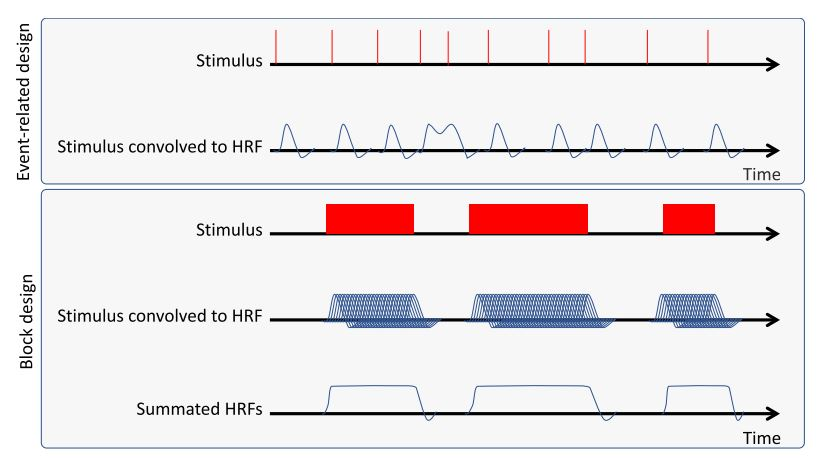
\includegraphics[width=.8\textwidth]{figures/aBackground/event_vs_block}  
	\caption{The top image show the event-related stimuli design and the stimulus convolved with the hemodynamic response function. The lower image depicts a block design, the stimulus convolved with hemodynamic response function and the summated HRF response.  \cite{Moayedi2018}}
	\label{fig:back:e_vs_b} 
\end{figure}

 



\section{Independent Component Analysis} \label{sec:ICA}
Independent component analysis has proven to be a very useful tool in separating noise from wanted signal in many applications. The following section will seek to elucidate the general basic theoretical background behind the blind source separation analysis.  

The basic idea about Independent Component Analysis (ICA) is to recover $m$ signal sources, which are mixed in $n$ observed signals. The observed signal is given by \cite{Hyvarinen2001}:
\begin{equation}
\mathbf{x} = \mathbf{A}\mathbf{s}
\end{equation}
where \textbf{x} is a observed signal vector containing the mixed signal elements $x_1, x_2, ..., x_n$, \textbf{s} is the source signal vector with the elements $s_1, s_2, ..., s_m$ and $\mathbf{A}$ is a mixing matrix with the dimension $n \times m$. Note that the dimensions of the mixing matrix can be equal to each other, meaning that it is required to have at least the number of observed signals as the source signals. The observed signal is assumed to be a linear mix of independent source signals. When performing ICA the goal is to find an inverted mixing matrix \textbf{$A^{-1}$} that recovers the source signal \cite{Hyvarinen2001}:
\begin{equation}
\mathbf{s} = \mathbf{A^{-1}}\mathbf{x}
\end{equation}
This can easily be achieved if the mixing matrix is known. However, this is rarely the case, as both the mixing matrix and source signals are unknown. There is no reliable way, to fully determine \textbf{s}, thus a set of assumptions are required, which the ICA method is based on \cite{Hyvarinen2001}:
\begin{itemize}
	\item The independent components (IC)’s are assumed to be statistically independent.
	\item The IC’s must be non-Gaussian distributions.
\end{itemize}
Regarding the assumption of independence, a set of variables $y_1, y_2, ..., y_n$ is not allowed to share mutual information so that $i \neq j$. This can be expressed as the joint probability of the variables is equal the product of each marginal probability of the variables \cite{Hyvarinen2001}:
\begin{equation}
p(y_1, y_2, …, y_n) = p(y_1) \cdot p(y_2) \cdot ... \cdot p(y_n) 
\end{equation} \label{eq:independence}
Satisfying this condition assures independency of the variables. A graphical example of independence in two dimensions is shown in \figref{fig:back:independence} \cite{Hyvarinen2001, Hyvarinen2000}. 

\begin{figure}[H]                 
	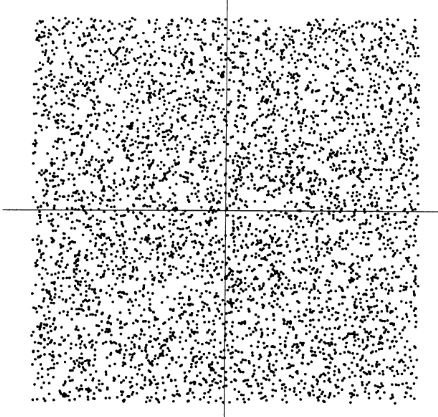
\includegraphics[width=.35\textwidth]{figures/aBackground/independence}  
	\caption{Figure illustrating the joint distribution of two independent components having uniform distribution. \cite{Hyvarinen2000}.}
	\label{fig:back:independence} 
\end{figure}

It is clear to see that information about a variable on the horizontal axis does not give any information about variables at vertical axis and vice versa.  Note that uncorrelatedness does not equal independency. However, whitening of the observed signals and thus ensuring uncorrelatedness is very helpful in solving the ICA problem. Whitening of the data is archived by performing a linear transformation that transforms the components so that the covariance matrix equals the identity matrix, thus having unit-variance. 
This can be expressed through performing a linear transformation of \textbf{x} into a random vector \textbf{z}:

\begin{equation}
\mathbf{z} = \mathbf{V}\mathbf{x} = \mathbf{V}\mathbf{A}\mathbf{s} 
\end{equation}
A graphical example of whitened data in two dimensions is shown in \figref{fig:back:whitening}  \cite{Hyvarinen2001,Hyvarinen2000}.

\begin{figure}[H]                 
	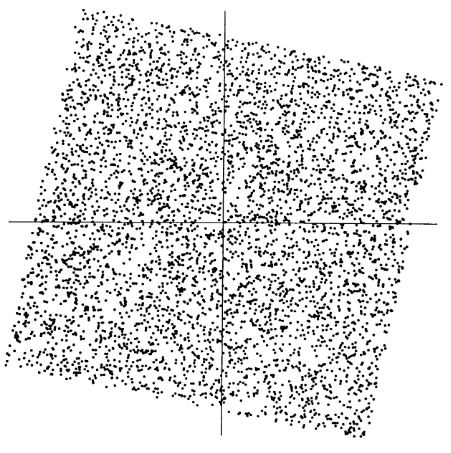
\includegraphics[width=.35\textwidth]{figures/aBackground/whitening}  
	\caption{Figure illustrating the impact of whitening on the joint distribution of two components \cite{Hyvarinen2000}.}
	\label{fig:back:whitening} 
\end{figure}

The squared distribution is clearly a rotated form of the independent data. What is left to ensure independence and solving the ICA problem is to estimate an angle that gives the correct rotation.
Concerning the second assumption on non-Gaussianity, the joint distribution of uncorrelated Gaussian distributions are not necessarily independent, and the distribution will be symmetrical and no information on the direction of the distribution can be derived. Thus, no transformation that allows independency can be performed, and the mixing matrix \textbf{A} can not be estimated from the mixtures. This can be shown in a two dimensional example with two sources $s_1$ and $s_2$ and the mixing matrix \textbf{A}, the joint probability density function (pdf) of Gaussian distributions is calculated as \cite{Hyvarinen2001}:
\begin{equation} \label{using this?}
\begin{split}
p(s_1,s_2) & = \frac{1}{2\pi}exp(-\frac{s^{2}_{1}+s^{2}_{2}}{2}) \\
& = \frac{1}{2\pi}exp(-\frac{\parallel \mathbf{s} \parallel ^2}{2}) 
\end{split}
\end{equation}
%\begin{equation}
%p(s_1,s_2) = \frac{1}{2\pi}exp(-\frac{s^{2}_{1}+s^{2}_{2}}{2}) 
%\end{equation}
%\begin{equation}
%= \frac{1}{2\pi}exp(-\frac{\parallel \mathbf{s} \parallel ^2}{2}) 
%\end{equation}
For an orthogonal mixing matrix \textbf{A} the inverse can be written as $\mathbf{A^{-1}} = \mathbf{{A^T}}$, and then $\mathbf{{s} = \mathbf{A^T} \mathbf{x}}$. The joint pdf can then be rewritten as:
\begin{equation}
p(x_1,x_2) = \frac{1}{2\pi}exp(-\frac{\parallel \mathbf{A^T} \mathbf{x} \parallel ^2}{2}) \mid Det (\mathbf{A^T}) \mid
\end{equation}
Because ${\parallel \mathbf{A^T} \mathbf{x} \parallel ^2} = \parallel \mathbf{x} \parallel ^2$ and $\mid Det ( \mathbf{A^T} ) \mid = 1$, hence the orthogonality of \textbf{A}, the joint pdf is:
\begin{equation}
p(x_1,x_2) = \frac{1}{2\pi}exp(-\frac{\parallel \mathbf{s} \parallel ^2}{2}) 
\end{equation}
The joint pdf is not changed when choosing an orthogonal mixing matrix as well as the property of independence. No further information about the mixing matrix can thus be revealed when the source signals are from a Gaussian distribution. \cite{Hyvarinen2001}

\subsection{ICA approaches}
As the mixing matrix and source signal most often are unknown, the IC’s must be approximated in an iterative process. There are two main ICA iteration approaches: minimizing mutual information and maximizing non-Gaussianity. The former approach seeks to minimize mutual information by maximizing independence between components. In practice this is done by minimizing the difference between the joint density distribution and the product of the marginal density functions, the left-hand side and right-hand side of \eqref{eq:independence}. This can for instance be done through a Kullback-Leibler divergence between the $p(y_1,y_2)$ and $p(y_1)*p(y_2)$ in a two dimensional case.
The second approach seeks to maximize non-Gaussianity of the components. The central limit theorem states that if sources are mixed, the mix tend to get more Gaussian than the individual sources. The strategy here is to find the directions in the data that is as far away from Gaussian as possible through a linear transformation. That direction will most likely be independent components. To find these directions different ICA approaches use fourth order moments and negentropy of the data. \cite{Hyvarinen2001} 
%
%\subsection{FastICA}
%For a single session ICA the MELODIC FSL program utilizes the FastICA algorithm to obtain independent components. This section seeks to lay out how the FastICA algorithm works and which mathematical techniques that are exploited. \\
%As stated in \secref{sec:ICA}, from the central limit theorem we get that observed mixed signals tend to have a more Gaussian distribution than the individual source signals, since the observed signal is a summation of the source signals. As a result of this, an approach is to find a linear transformation that leaves the source signals as non-Gaussian as possible. This principle is what the FastICA algorithm is build up around. \\
%Firstly the vector \textbf{b} is introduced, which is a row vector in the mixing matrix \textbf{A}, and is used in a linear combination:
%
%\begin{equation}
%y = \mathbf{b^T}\mathbf{x}
%\end{equation}
%
%By substituting $\mathbf{x} = \mathbf{A}\mathbf{s}$ in the previous equation:
%
%\begin{equation}
%y = \mathbf{b^T}\mathbf{A}\mathbf{s} = \mathbf{q^T}\mathbf{s}
%\end{equation}
%
%Where $\mathbf{q^T} = \mathbf{b^T}\mathbf{A}$. From this it can be deduced that \textit{y} is an IC, when only one of the entries of \textbf{q} is non-zero and the rest is zero. This means that there is no addition of any random processes and the component will be as non-Gaussian as possible. An IC can then be obtained by calculating a value of \textbf{b} that maximizes the non-Gaussianity of the distribution of $\mathbf{b^T}\mathbf{x}$ as $\mathbf{b^T}\mathbf{x} = \mathbf{q^T}\mathbf{s}$. This gives an optimization problem with convergence at local maxima. As there exist a local maximum of the non-Gaussianity for both \textit{s} and ${s_i}$, the optimization landscape in a n-dimensional signal gives a total of \textit{2n} local maxima.
%To be able to optimize according to non-Gaussianity, a quantitative measure of such is needed. This can be provided by the fourth order cumulant, kurtosis, which is zero when \textit{y} is Gaussian distributed and non-zero when \textit{y} is non-Gaussian distributed (negative when sub-Gaussian and positive when super-Gaussian). Given this property and the central limit theorem, the linear combination $\mathbf{b^T}\mathbf{x}$ that yields an IC can be found at the local maxima of the absolute value of the kurtosis of \textit{y}. The kurtosis of \textit{y} is given by:
%		
%\begin{equation}
%kurt(y) = E{y^4} - 3E{y^2}^2
%\end{equation}
%	
%As the whitening of the data results in unit-variance, \textit{kurt(y)} can be modified to:
%		
%\begin{equation}
%kurt(y) = E{y^4} - 3
%\end{equation}
%		
%To simplify the theoretical analysis furthermore the linear properties of kurtosis for sums of variables can be utilized. For two random variables, \textit{$x_1$} and \textit{$x_2$}, it holds that:
%	
%\begin{align*}
%kurt(x_1 + x_2) &= kurt(x_1) + kurt(x_2)
%kurt(\alpha x_1) &= \alpha^4 kurt(x_1)
%\end{align*}
%	
%For the multiplicative scalar \textit{$\alpha$} the kurtosis is non-linear, and the optimization problem can thus be written as:
%			
%\begin{equation}
%kurt(y) = \sum_{i} q_{i}^{4}kurt(s_i)
%\end{equation}
%			
%Due to the whitening of the data, where \textit{y} has unit-variance, a constraint is put on the vector \textbf{q}. Since $E{y^2} = \sum_{i}^{n} q_{i}^{4}$ the vector \textbf{q} is constrained to the unit-sphere. For the whitened data \textbf{z} a linear combination $\mathbf{w^T}\mathbf{z}$ that maximizes non-Gaussianity is sought for. From the fact that $\mathbf{q} = \mathbf{V}\mathbf{A})^{T}\mathbf{w}$, the following is given:
%			
%\begin{equation}
%\parallel \mathbf{q} \parallel^{2}= (\mathbf{w}^{T}\mathbf{V}\mathbf{A})(\mathbf{A}^{T}\mathbf{V}^{T}\mathbf{w}) = \parallel \mathbf{w} \parallel^{2}
%\end{equation}
%			
%This expresses that constraining the vector \textbf{q} to lie on the unit sphere equally constraints \textbf{w} to the unit sphere. The objective is now to find a value of \textbf{w} that maximizes the absolute value of the kurtosis of $\mathbf{w^T}\mathbf{z}$. Whitening further allows the linear combination $\mathbf{w^T}\mathbf{z}$ to be understood as projections on the line in a 1-D subspace spanned by \textbf{w}. What is sought for is the direction of \textbf{w} where the absolute value is maximized, which then makes out an IC. \\
%To solve this optimization problem a commonly used technique is the gradient algorithm to reach convergence at local maxima, thus calculating the direction where the absolute value of the kurtosis of $\mathbf{w^T}\mathbf{z}$  is growing most strongly. The can be computed as the following:
%			
%\begin{equation}
%\frac{|kurt(\mathbf{w^T}\mathbf{x})|}{\mathbf{w}} = 4sign(kurt(\mathbf{w^T}\mathbf{z})[E{\mathbf{z}(\mathbf{w^T}\mathbf{z})^{3} - 3\mathbf{w}\parallel\mathbf{z}\parallel ^{2}}
%\end{equation}
%				
%However, there is in practice disadvantages associated with using the gradient algorithm, e.g. slow convergence rate and is dependent on a proper choice of learning rate. The fixed point algorithms is suggested as a faster algorithm alternative. At the stable point of the gradient algorithm, the gradient is pointing the direction of \textbf{w}. It is only in this case that \textbf{w} will not change direction when adding the gradient. This notion about the gradient of the absolute value of the kurtosis can be used to form a fast fixed point algorithm, or the FastICA algorithm:
%
%Ligning og tekst udkommenteret	
%%\begin{equation}
%%\textbf{w} \leftarrow$  E{\textbf{z}{\textbf{w^{T}\textbf{z}}^3} - 3\textbf{w}}
%%\textbf{w} \leftarrow \textbf{w} / \parallel \textbf{w} \parallel
%%\end{equation}
%%					
%%The right hand side is firstly computed and assigned to \textbf{w}, which afterwards is normalized to follow the constraint of $\parallel \mathbf{w} \parallel ^2 = 1$. By iterating over this convergence is reached at an ultimate \textbf{w}, where $\mathbf{w^T\mathbf{z}$ is an IC. In order to obtain several IC’s the process is repeated, with the constraint that \textbf{w} must be orthogonal to all previously computed \textbf{w}. 
%



\section{Principal Component Analysis}

The use of principal component analysis (PCA) in denoising algorithms has been exploited in various studies, showing that the properties of the PCA might be useful \cite{Behzadi2013}. In this section the theory and common use of PCA is presented, including a small part on its use in images. 

Principal Component Analysis (PCA) is a well renowned and widely used analysis tool, capable of finding the most defining variables in a dataset. This facilitates finding the components that are the most saying for the dataset. This introduces the possibility of dimensionality reduction by lowering the amount of redundant information. The PCA is used to transform a set possibly correlated variables into a set of uncorrelated components, called principle components. Each principal component (PC) is
orthogonal on the former and are uncorrelated and have zero covariance. They each define the largest
variance in an axis, such that PC 1 describes the direction of the maximum variance of the dataset. Each
following PC describes the next highest variance of the dataset, with the constraint that it is orthogonal
and has zero covariance with any of the former PCs. PCA is the orthogonal projection of data onto a
lower dimension linear space.  A PC is found by minimizing the variance by projecting the feature values (blue dots) onto the line (now red dots) describing the highest variance in the data set (black line) as seen on \figref{projection}. The PC is found by minimizing the mean square distance between the data points. \cite{Semmlow2004}

\begin{figure}[H] 
	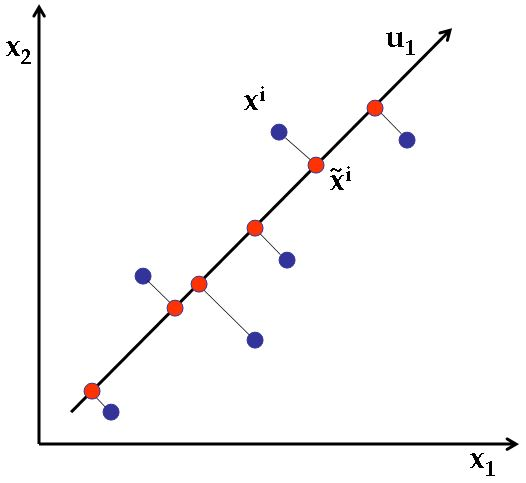
\includegraphics[width=0.38\textwidth]{figures/aBackground/projection}
	\caption{Two-dimensional example of projection of data variables (blue dots) onto a PC axes (black line). $(u_1)$ indicates the direction of the eigenvector. \cite{PCA2018}}
	\label{projection}
\end{figure}

The algebraic method of calculating the PCs can be done by using Singular Value Decomposition (SVD). The first step is to compute the squared cross product matrix of variances and covariances among every pair of the variables in the data set, where the diagonals are the variances and the off-diagonals are the covariances, as done in the following equation:
%\vspace{-20pt}
\begin{equation}
S = X \textquoteright X
\end{equation}
Where S is the cross product and X is the dataset matrix. When finding the PCs it includes an eigen-analysis of S. The eigenvalues of are solutions to the following equation:
%\verticalspace{1}
\begin{equation}
| S - \lambda I |  = 0
\end{equation}
Where $\lambda$ is the variances of each PC and I is the identity matrix. After solving for $\lambda$ the eigenvectors can be solved through the following equation:
\begin{equation}
det | S - \lambda I | b_{i} = 0
\end{equation}
Where $b_{i}$ is used to calculate the eigenvectors as in:
\begin{eqnarray}
u_{i} = \frac{b_{i}}{\sqrt{b_{i}^{\textquoteright} b_{i}}}
\end{eqnarray}
Where $u_{i}$ is the $i$ number of eigenvectors that contain a contribution to the principal components.
The SVD orders the eigenvalues by size $\lambda_{1} > \lambda_{2} … > \lambda_{i}$. The scores for each PC is equal to the corresponding eigenvalue for that exact axis. The eigenvalues describe how much of the variance is accounted for by the associated PC. Summation of all eigenvalues accounts for the total variance of the data set; this is called the trace. To find how much the each PC accounts for, the eigenvalue of that PC is divided by the total variance: $\%~ of~ total~ variance~ = \frac{\lambda_{i}}{Trace}$. This can be used for deciding how many components are significant and by how much the dataset can be reduced. \cite{Semmlow2004}

\subsection{PCA in images}

The PCA can also be implemented on images, where the dimensionality reduction principle is mostly used for image compression. Here images can be reconstructed using only very few principle components without much information loss. Similarly PCA can be used to de-noise images, as noise would be presented in some of the less saying components, and by removing these, noise would be removed from the image. \\
The PCA can be run on the entire image, but methods introducing local PCA in smaller windows of the image, have also been introduced for noise removal. \cite{MuraliMohanBabu2012}   



%\section{General Linear Model} \label{back:sec:glm}

In order to determine if a task or stimuli has made a significant contribution to the measured BOLD signal, each voxel in the scan needs to be evaluated. The following section will therefore seek to explain a method of how to determine if any significant change is found. In this project the general linear model (GLM) will be explained and applied as it is the most used and recognized tool for fMRI analysis during the past 20 years \cite{Poline2012}. 

The GLM is a well considered and used analysis tool constituting a simple way of doing standard statistical analysis on fMRI. The overall goal of the GLM model is to determine how well the time course of the scan corresponds to the known used experimental interference.  In an fMRI case, that means, how well the BOLD signal over time fits the time course of the predicted signal given by the imposed stimuli, that causes brain activity. This statistical test is carried out for each voxel independently of its neighbor across the scan resulting in thousands of statistical tests in one scan. \cite{Moayedi2018,Monti2011} To explain the implementation of a GLM we can use the example presented by \cite{Monti2011}. An acquired BOLD signal will throughout a time series, of \textit{n} images, have a varying output signal. The signal in a voxel $Y$, at any time point, can be seen as a summation of predictor variables (regressors of interest) $X$ and nuisance regressors (regressors of none-interest) that model noise $X$, a scaling parameter for each regressor $\beta$, and an error term $\epsilon$. This can be presented in the GLM's basic from as \cite{Monti2011}: 
\begin{equation}
Y=X\beta+\epsilon
\end{equation}

Expanding this formulation into a complete scan, including multiple regressors, can be presented on a matrix form. A depiction of a GLM design matrix incorporating the factors making up the BOLD signal can be seen in \figref{fig:GLM}. 

\begin{figure}[H] 
	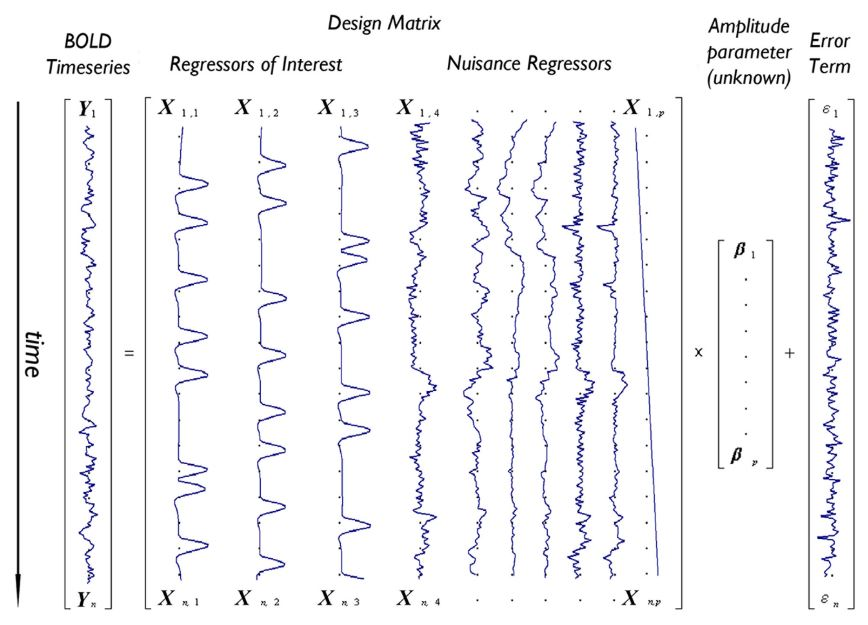
\includegraphics[width=0.90\textwidth]{figures/aBackground/GLM}
	\caption{Illustration of a design matrix for a given GLM model, describing the BOLD time series $Y_n$, the regressors of interest $X_{1,1}, X_{1,2}, X_{1,3}$, the nuisance regressors $X_{4..p}$, the amplitude parameter $\beta_{1..p}$ and the error terms $\epsilon_{1..n}$. Illustration taken from \cite{Monti2011}.}
	\label{fig:GLM}
\end{figure}



The predictor variables are found by modeling what is known or predicted as output. The predictors of interest would come from hemodynamic response curve convoluted with stimuli design as presented in \secref{sec:Stim}. GLM models will often introduce nuisance predictors as well used to model variables such low frequency drift and motion to make a more robust model. These are non interest regressors, as they do not resemble the wanted signal, being the stimuli induced. The amplitude parameter is the unknown weight, scaling the magnitude of resemblance between each predictor value and the output. They describe the strength of the relationship between that regressor and the voxel's BOLD signal course of activation. The error term contains the value for each observation, which can not be explained by the weighted sum of the amplitude parameter. \cite{Moayedi2018,Monti2011} 

The goal is to estimate the value of the scaling parameter $\beta$ for all regressors and afterwards determine if any regressor significantly account for the variance found in the BOLD signal. A regressor associated with the measured BOLD signal should hypothetically show a greater value for the voxels in the brain area corresponding to a given task. E.g. finger tapping would show greater $\beta$ values in the motor cortex. A method for estimating $\beta$ values for the regressors is the ordinary least squares (OLS). The OLS method estimates $\beta$ by minimizing the sum of squared residuals \cite{Monti2011}: 

\begin{equation}
\sum_{i=1}^{n}(Y_i-X_i\times\hat{\beta})^2
\end{equation}  

Y is the observed signal, X is the predicted signal which is scaled by $\beta$. $\beta$ and the variance of $\beta$ can be estimated by: 

\begin{equation}
\hat{\beta}=(X^TX)^{-1}X^TY
\end{equation}

\begin{equation}
var(\hat{\beta})=\sigma^2(X^TX)^{-1}
\end{equation}

The application of this method rests on the following assumptions being fulfilled: Error terms are independently and Gaussian distributed with zero mean, the regressors in the matrix are independent of error, non stochastic and known and no regressor is a linear transformation of another regressor. \cite{Monti2011}    






\end{appendices}


\end{document}
